%\section{Results for Alternative Likelihoods}\label{sec:alt_results}

% \subsection{Parameter Priors}\label{sec:priors}

% In this section we compare posteriors that use priors for black hole feedback, $\epsilon_{AGN}$, and the matter density, $\Omega_M h^2$, to our main results, which did not include parameter priors.
% From Planck \cite{2020A&A...641A...6P}, we have a prior for $\Omega_M h^2=0.1424\pm0.001$.
% The prior for the black hole feedback factor, $\epsilon_{AGN}$, is included to effectively remove this parameter from the inference, as it is not well constrained and does not have a strong effect on the flux power or mean temperature (the prior is $\epsilon_{AGN} = 0.05 \pm 0.01$).
% All priors are Gaussian and implemented in the likelihood.

% The chains are once again divided into redshift ranges, with one pair using $z=2.2-4.6$ and the other using $z=2.6-4.6$.
% Figure~\ref{fig:priors_corner} shows the results when using priors, as well as our main results without priors, for comparison.
% When we include the Planck prior on $\Omega_M h^2$ and the prior on $\epsilon_{AGN}$, all the other parameters are changed only marginally.
% This is encouraging, as our results are robust to the inclusion of priors, and the correlations between most sets of parameters are weak.
% The only parameter that does change is $h$, which for the full redshift range chain begins to develop a second mode in the posterior near $h=0.69$.
% This is likely due to the degeneracy between $h$ and $\Omega_M h^2$.

% \begin{figure}
%     \centering
%     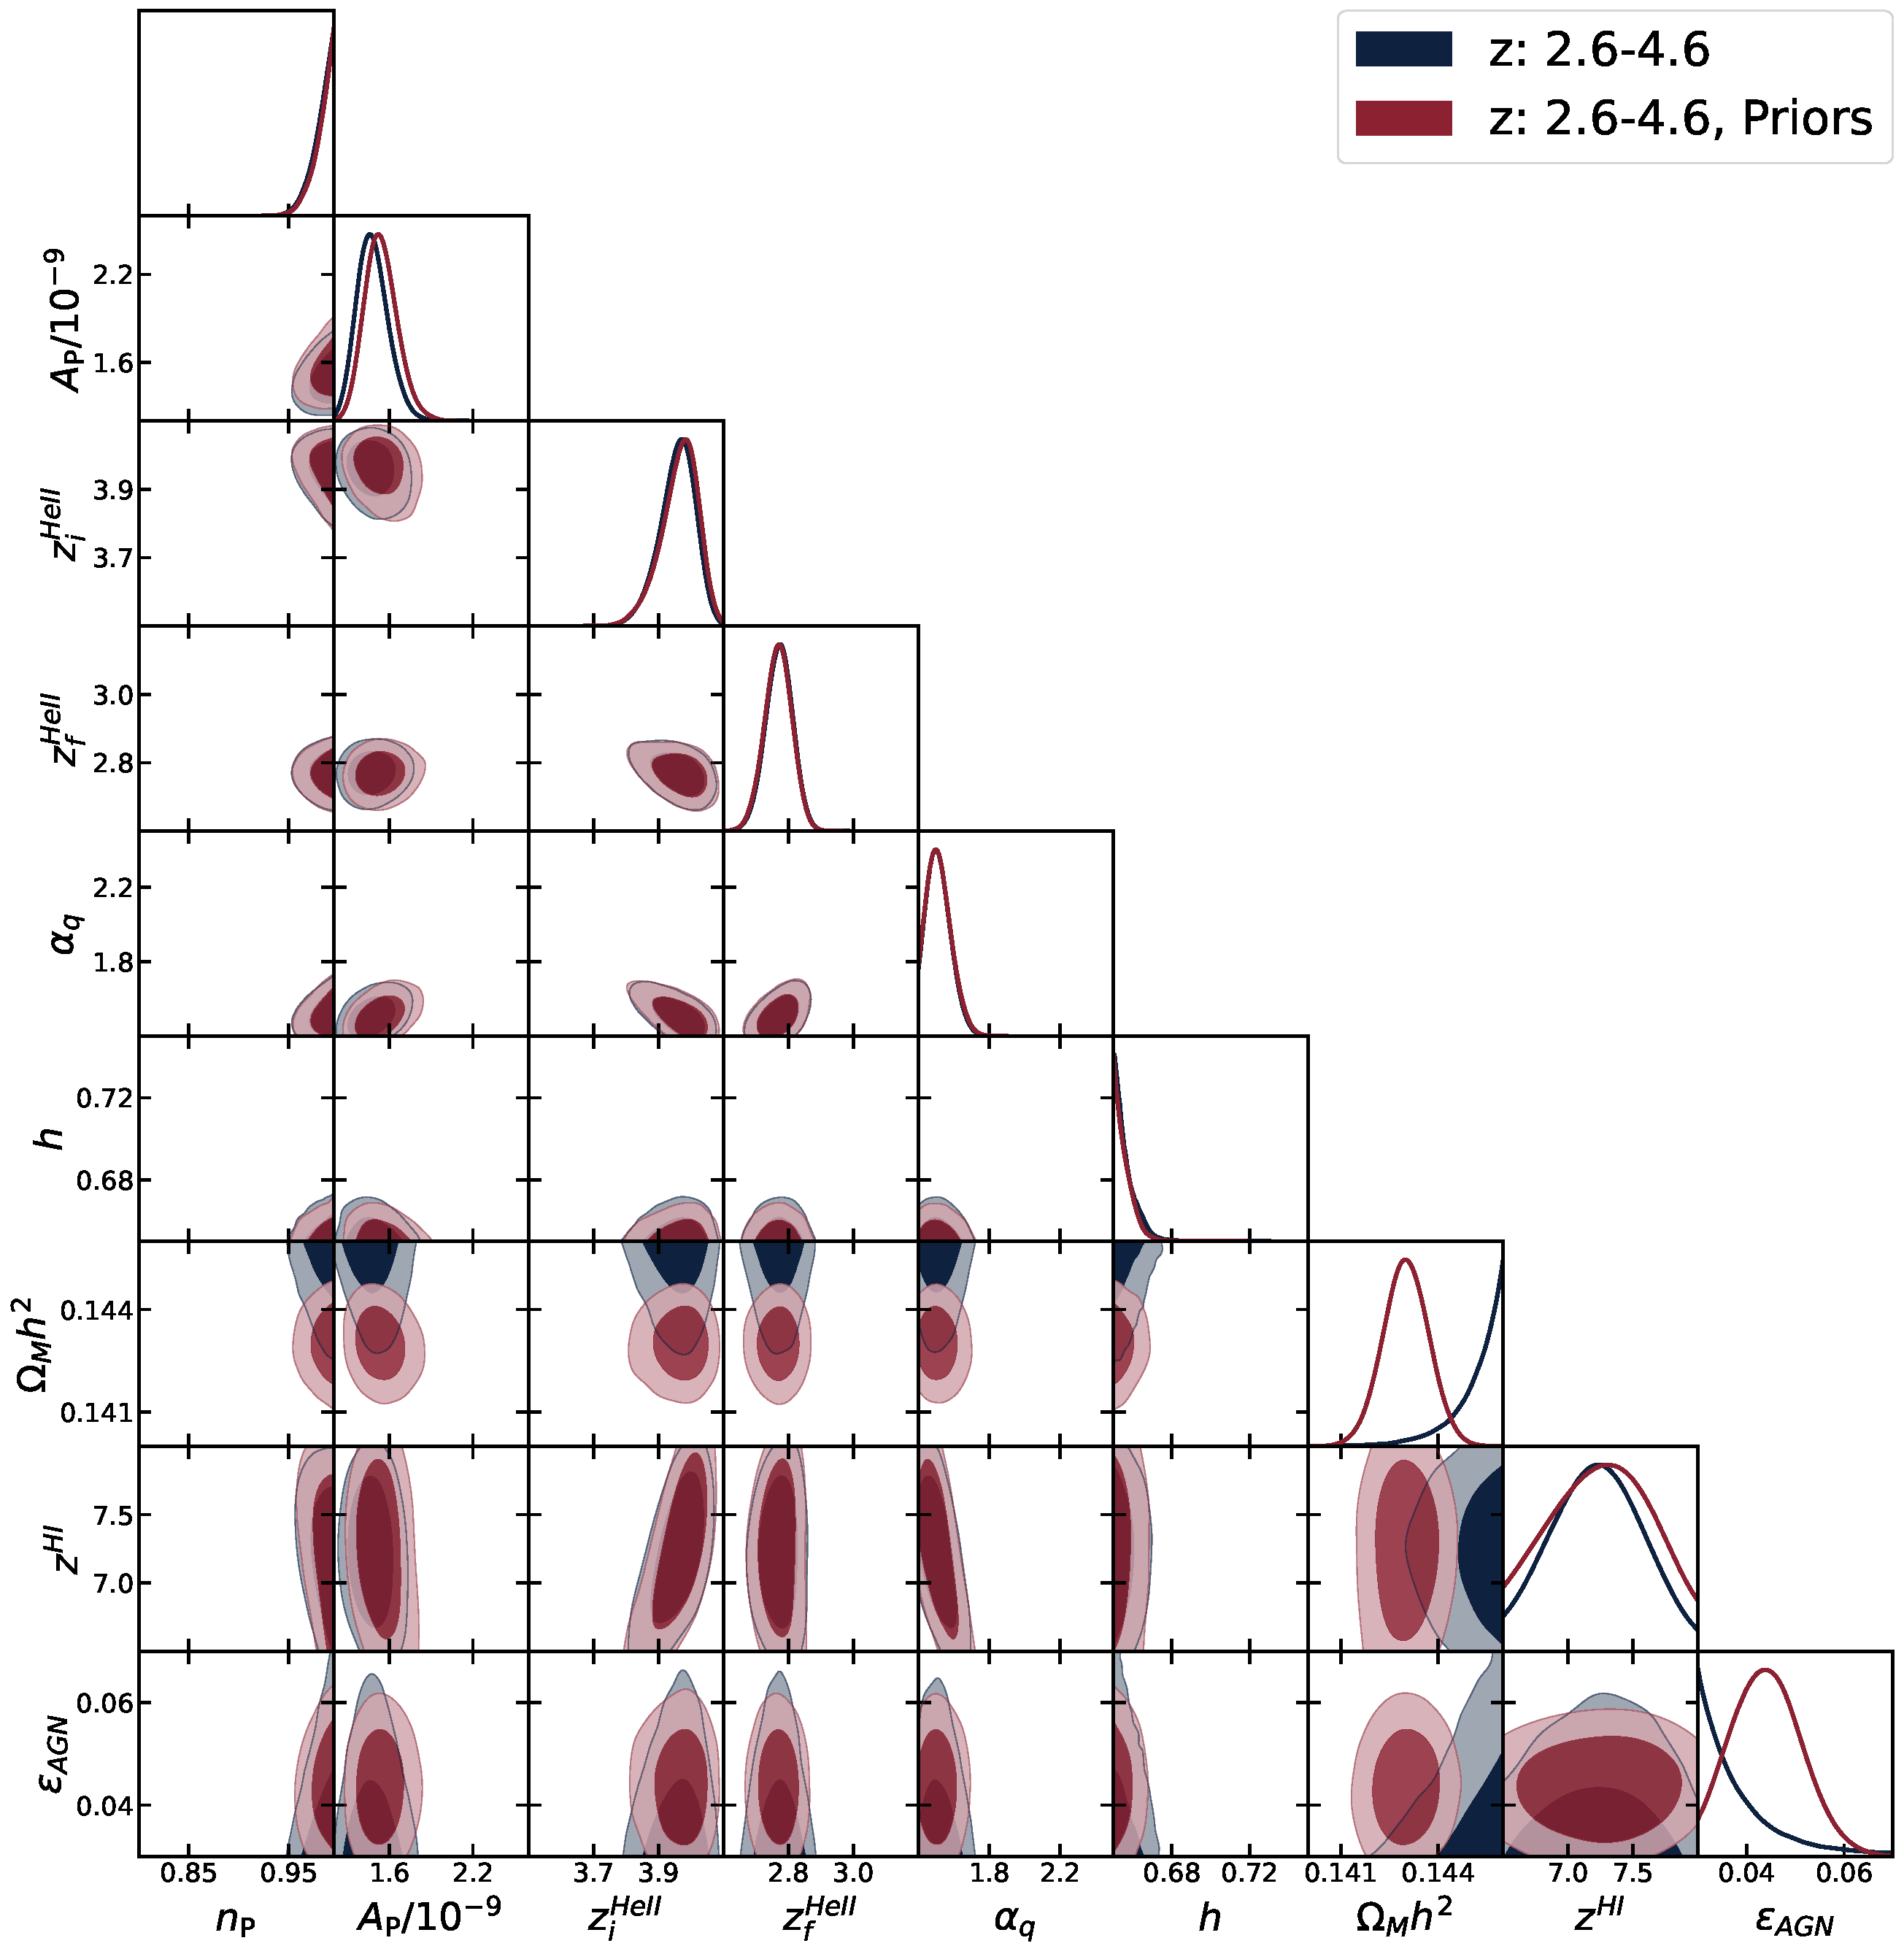
\includegraphics[width=\textwidth]{figures/priors.pdf}
%     \caption{\label{fig:priors_corner}
%     Posteriors for chains run using priors on $\epsilon_{AGN}$ and $\Omega_M h^2$ (red, blue), as compared with their counterparts run without priors (black, yellow).
%     }
% \end{figure}

% --------------------------------------------------------------------------------------------------
% --------------------------------------------------------------------------------------------------
% --------------------------------------------------------------------------------------------------
% --------------------------------------------------------------------------------------------------
% --------------------------------------------------------------------------------------------------

% --------------------------------------------------------------------------------------------------
% --------------------------------------------------------------------------------------------------
% --------------------------------------------------------------------------------------------------
% --------------------------------------------------------------------------------------------------
% --------------------------------------------------------------------------------------------------


\section{Leave-one-out versus Emulator Error}
\label{sec:loovsgperr}
\begin{figure}
    \centering
    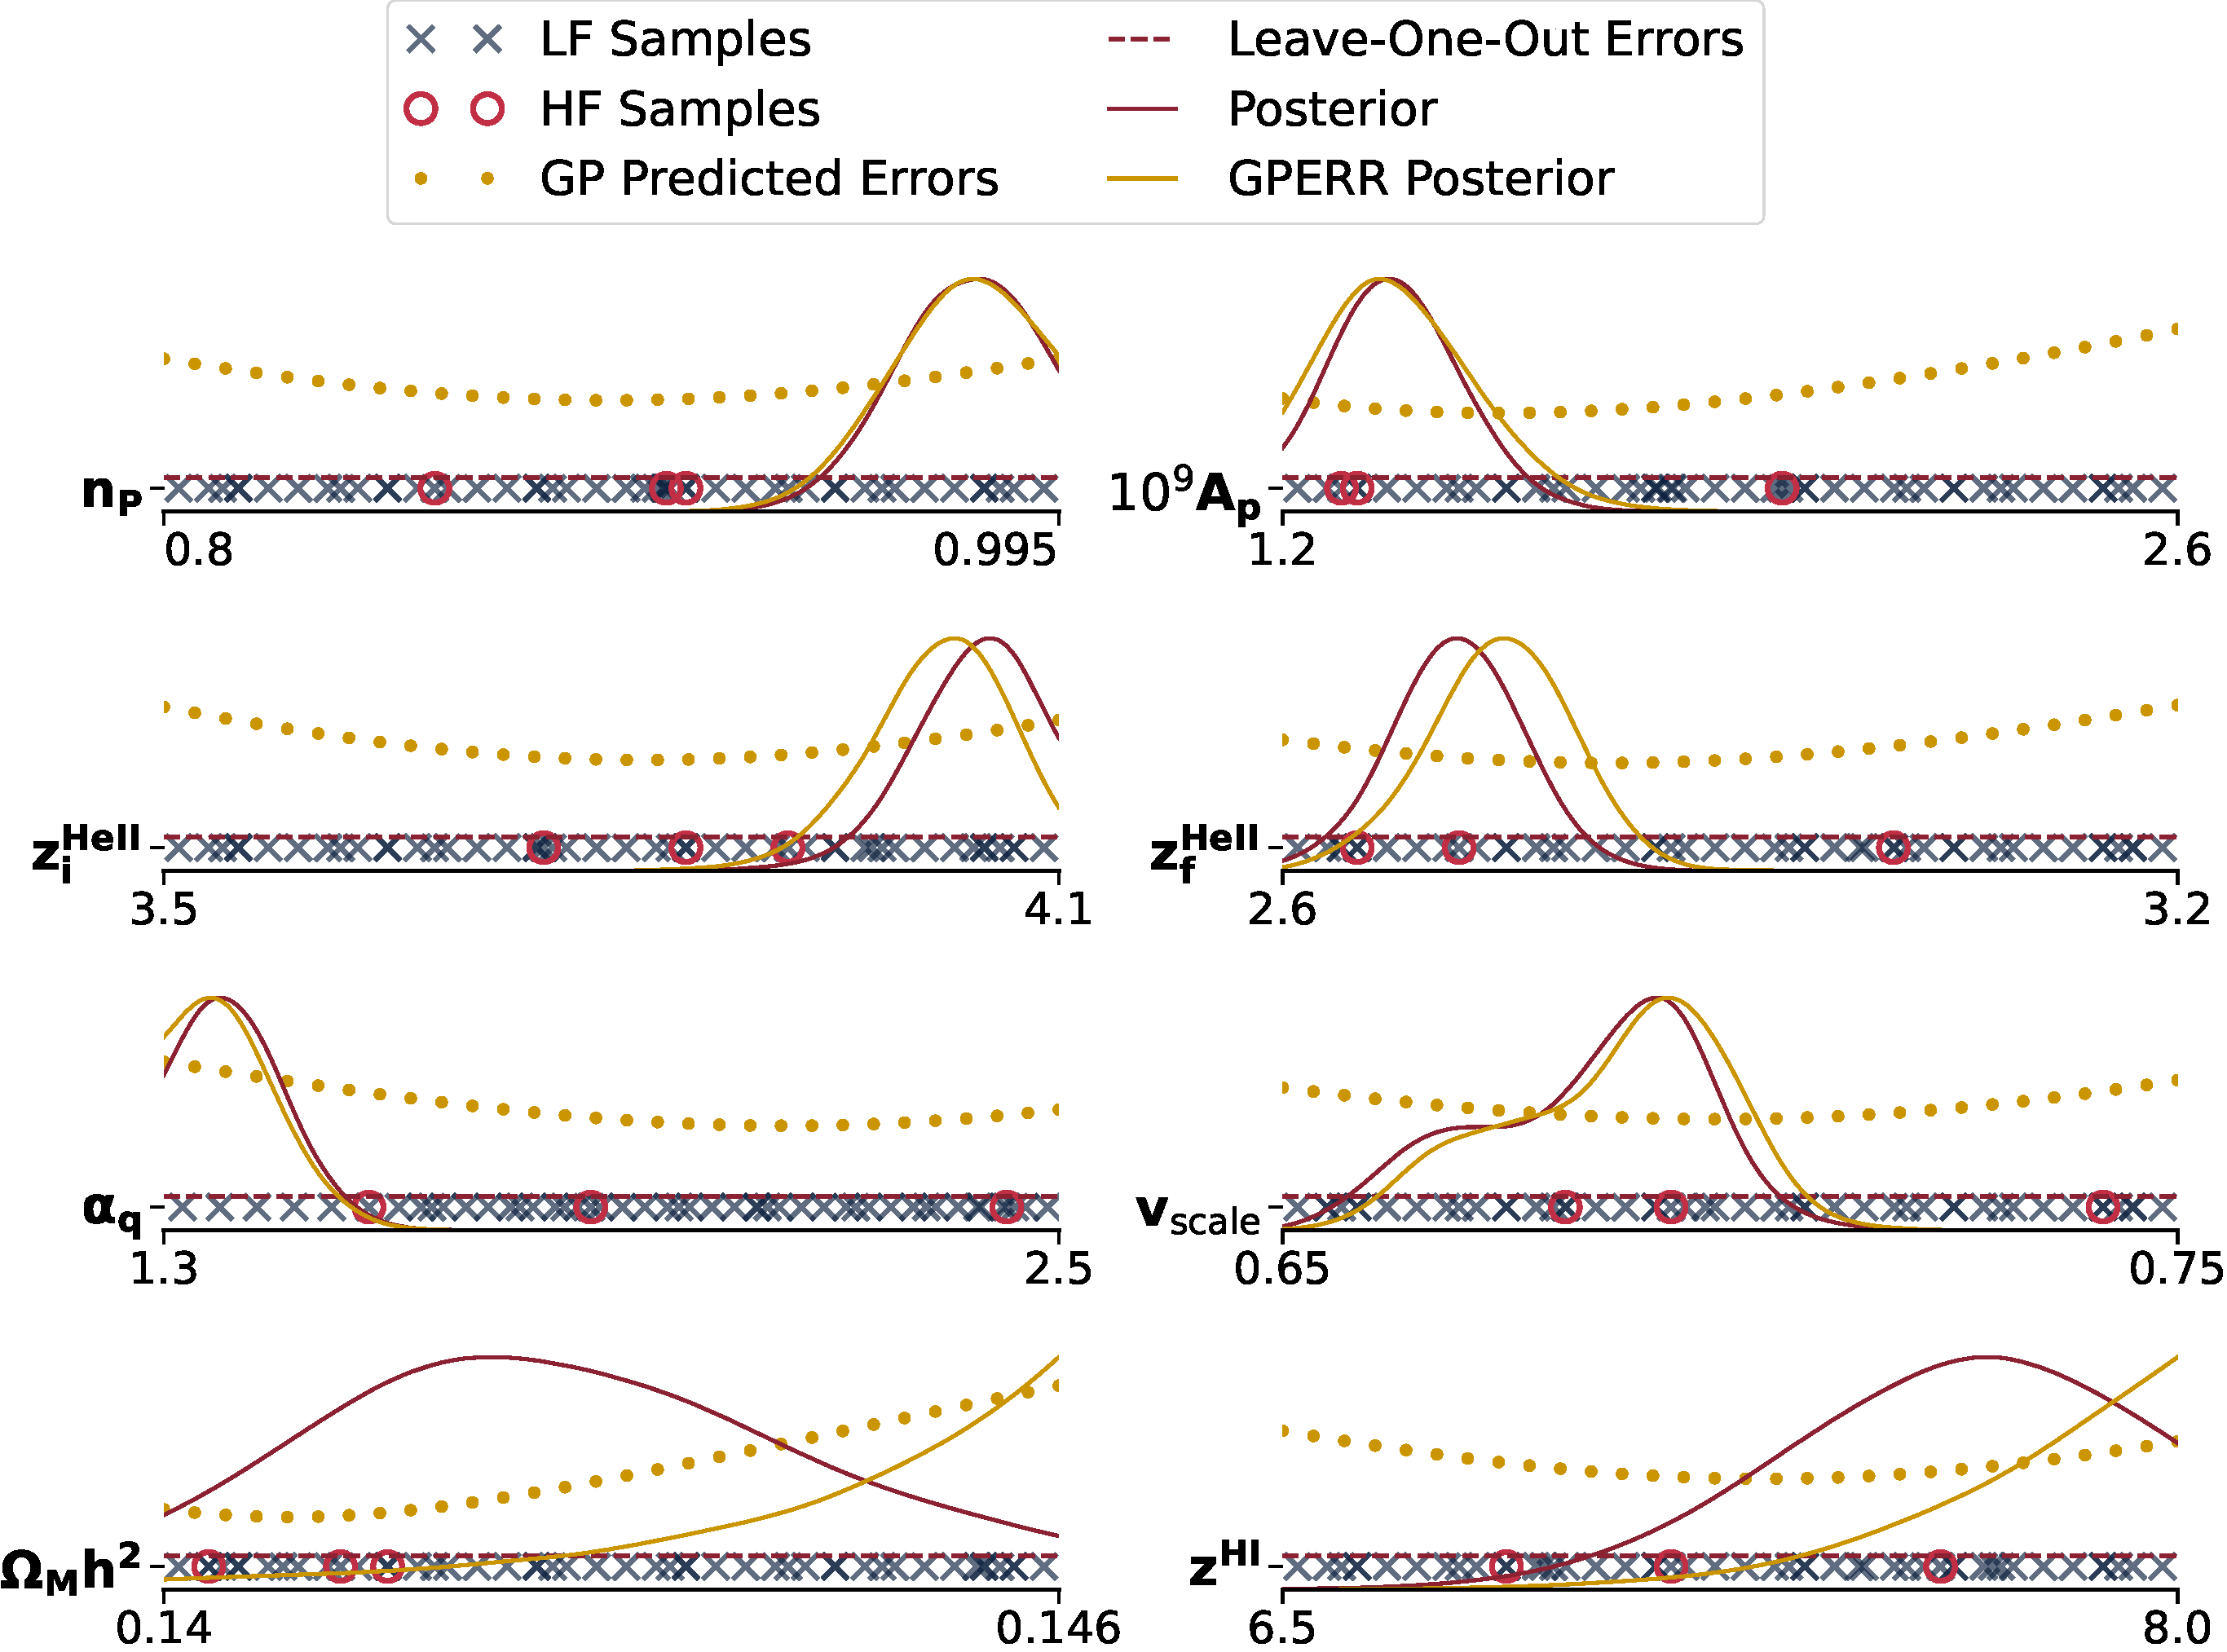
\includegraphics[width=\textwidth]{figures/loo_vs_emu_error_wlegend.pdf}
    \caption{\label{fig:loo_v_emu}
    Emulator error and leave-one-out errors across parameter space.
    For eight of the input parameters, the training samples (grey crosses for LF, red circles for HF), GP emulator errors (yellow dots), and scale-averaged leave-one-out errors (red dashed) are shown. All chains contain the IGM temperature data, and the eBOSS flux power spectrum from $z=2.6 - 4.6$.
    Shown are 1D marginalised posteriors for the chains with the default likelihood (red) compared to chains run adding the GP emulator error to the likelihood (yellow).
    }
\end{figure}

In this Appendix we evaluate the impact of including the Gaussian Process interpolation error, $\boldsymbol{\sigma}_{GP}$, on the posterior parameters, as discussed in Equation~\ref{eq:covariance}.
Figure~\ref{fig:loo_v_emu} compares the effect of including emulator errors, showing the training samples, GP emulator errors and scale-averaged leave-one-out errors.
The leave-one-out error is independent of position in parameter space, whereas the GP error is larger towards the edge of parameter space.
The largest effect is on the matter density $\Omega_M h^2$. With the GP error, helium reionization starts later and finishes earlier, as well as producing more heating. On the other hand, hydrogen reionization happens earlier. However, these shifts are all less than $1.5-\sigma$. The cosmological parameters are unchanged.
%\begin{figure}
%    \centering
%    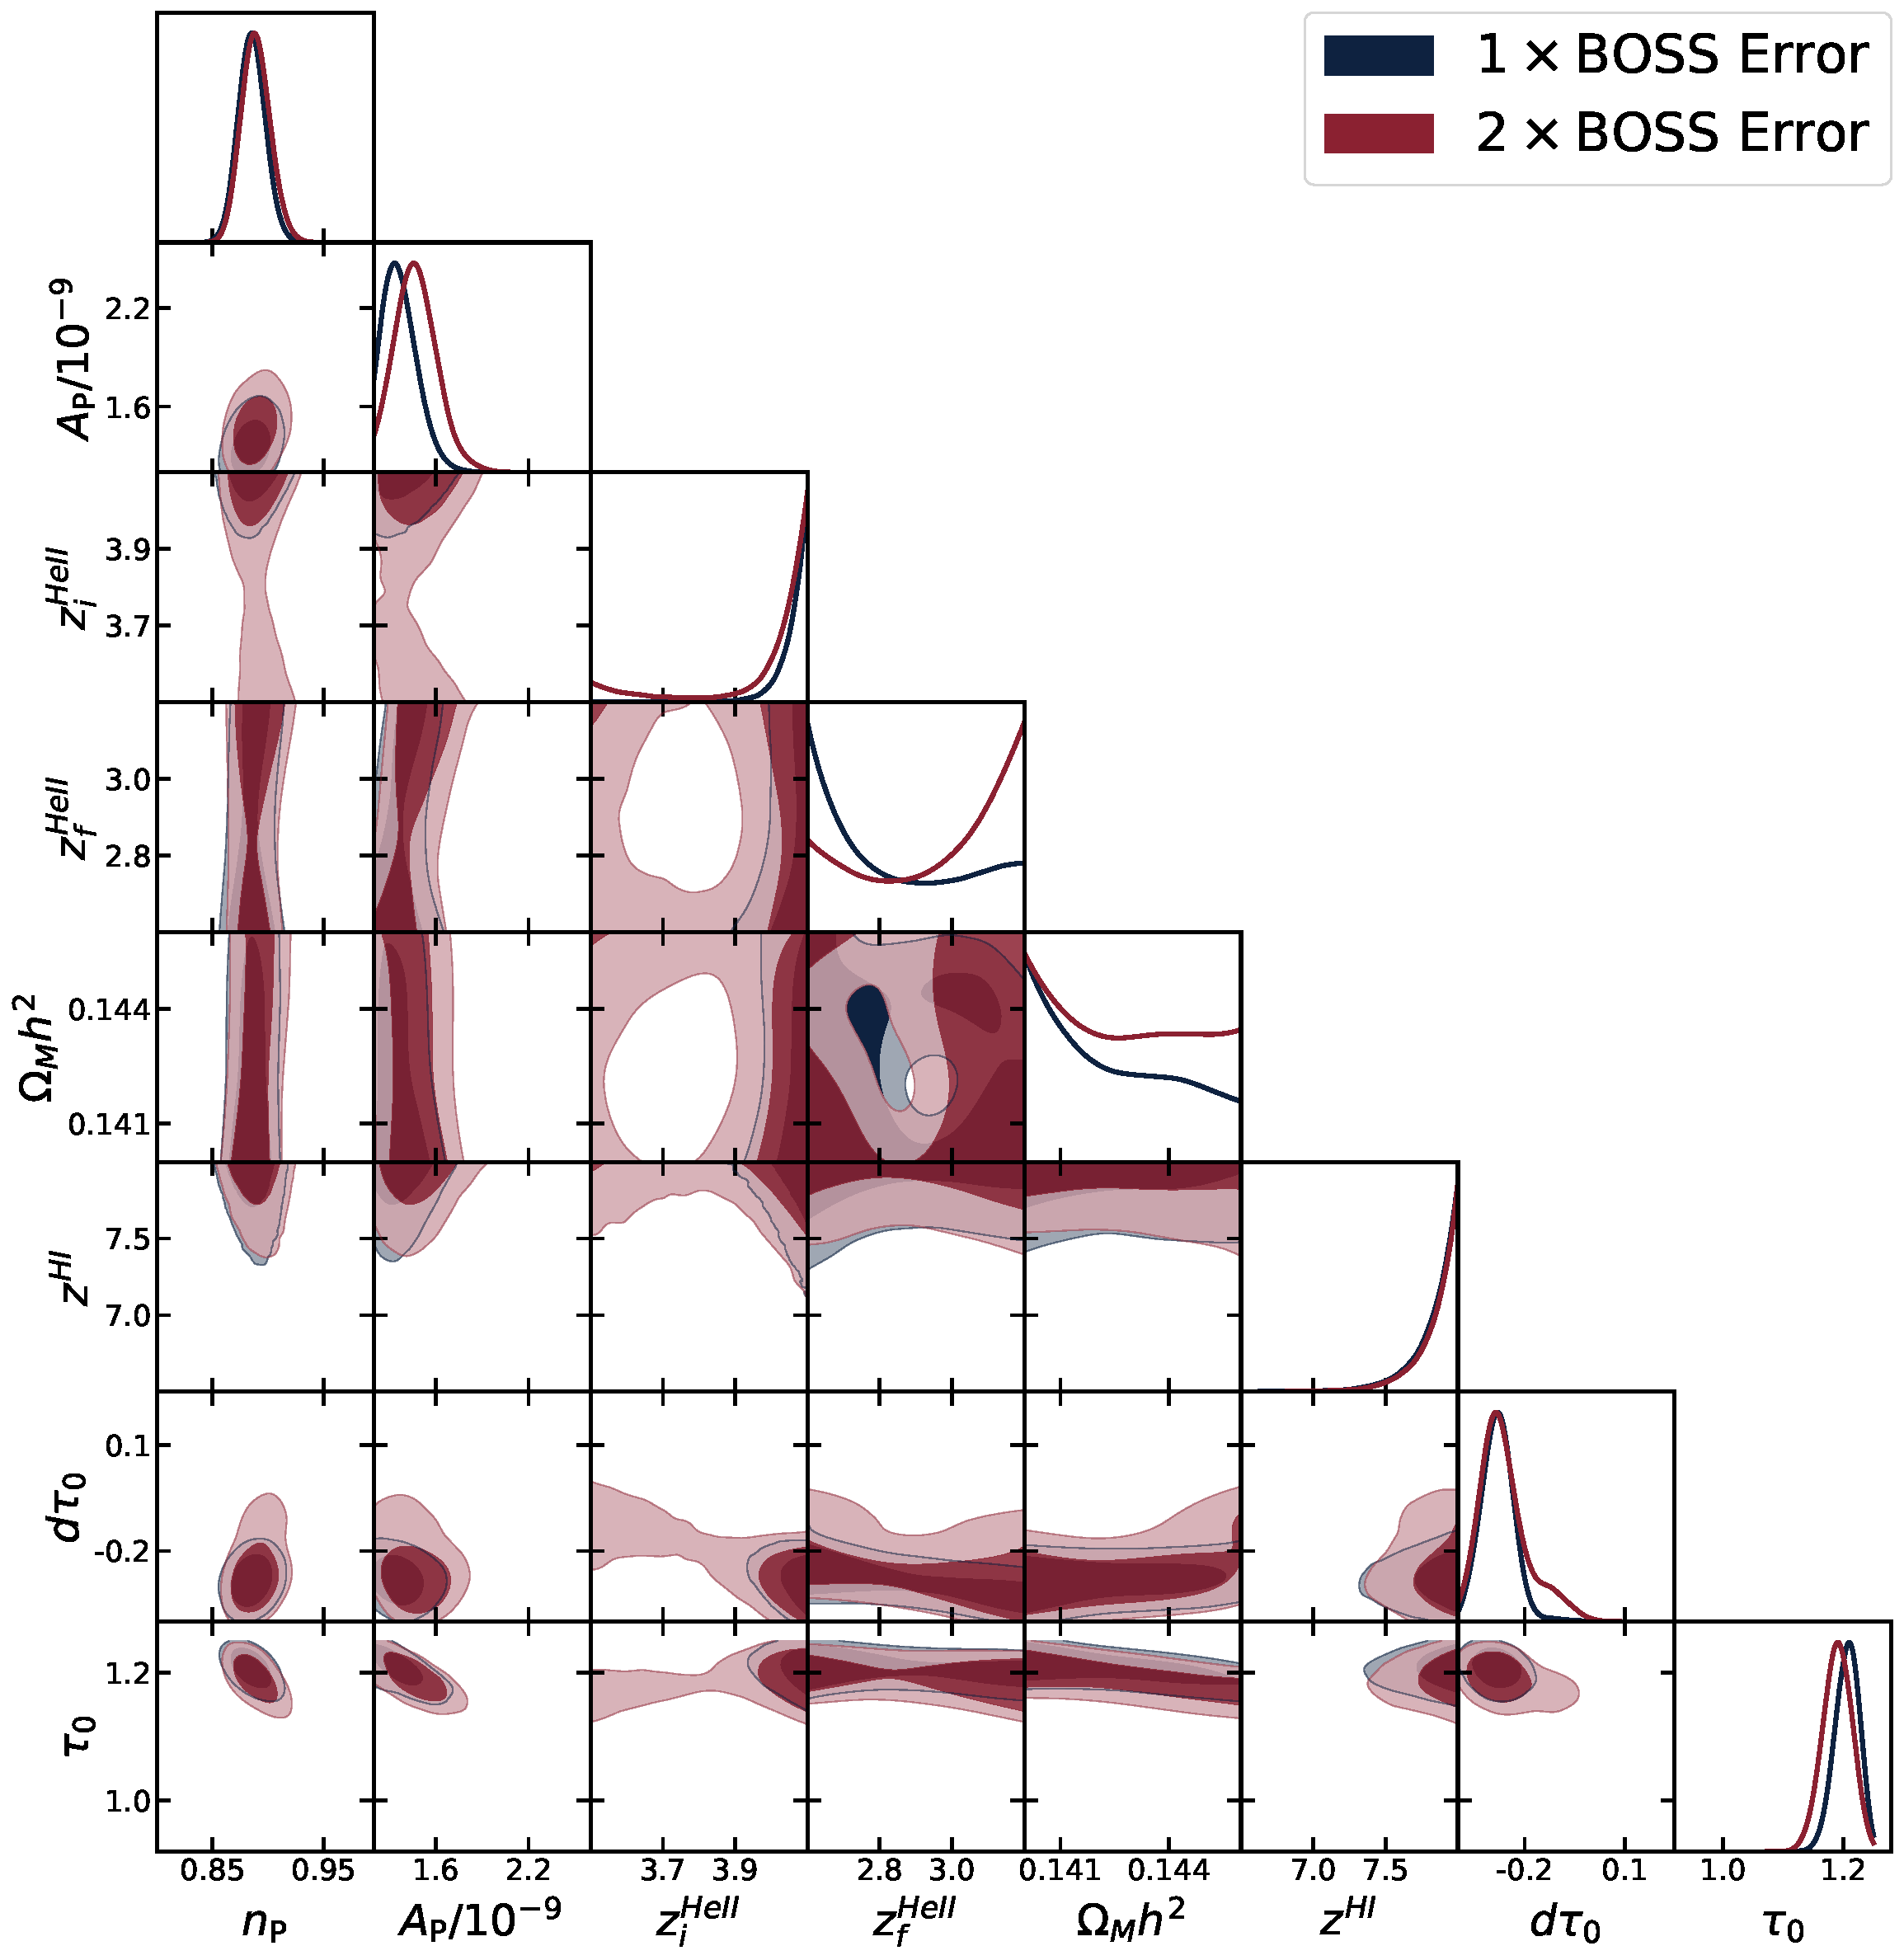
\includegraphics[width=\textwidth]{figures/2xboss.pdf}
%    \caption{\label{fig:2xboss_corner}
%    Posteriors for a chain run using observations with inflated errors: the default errors (black), root two times the default (red), and two times the default (yellow).
%    These use only the flux power, and include the full redshift range, $z=2.2-4.6$.
%    }
%\end{figure}


% --------------------------------------------------------------------------------------------------
% --------------------------------------------------------------------------------------------------
% --------------------------------------------------------------------------------------------------
% --------------------------------------------------------------------------------------------------
% --------------------------------------------------------------------------------------------------


% \subsection{Single-Fidelity Results}\label{sec:sf_results}

% \begin{figure}
%     \centering
%     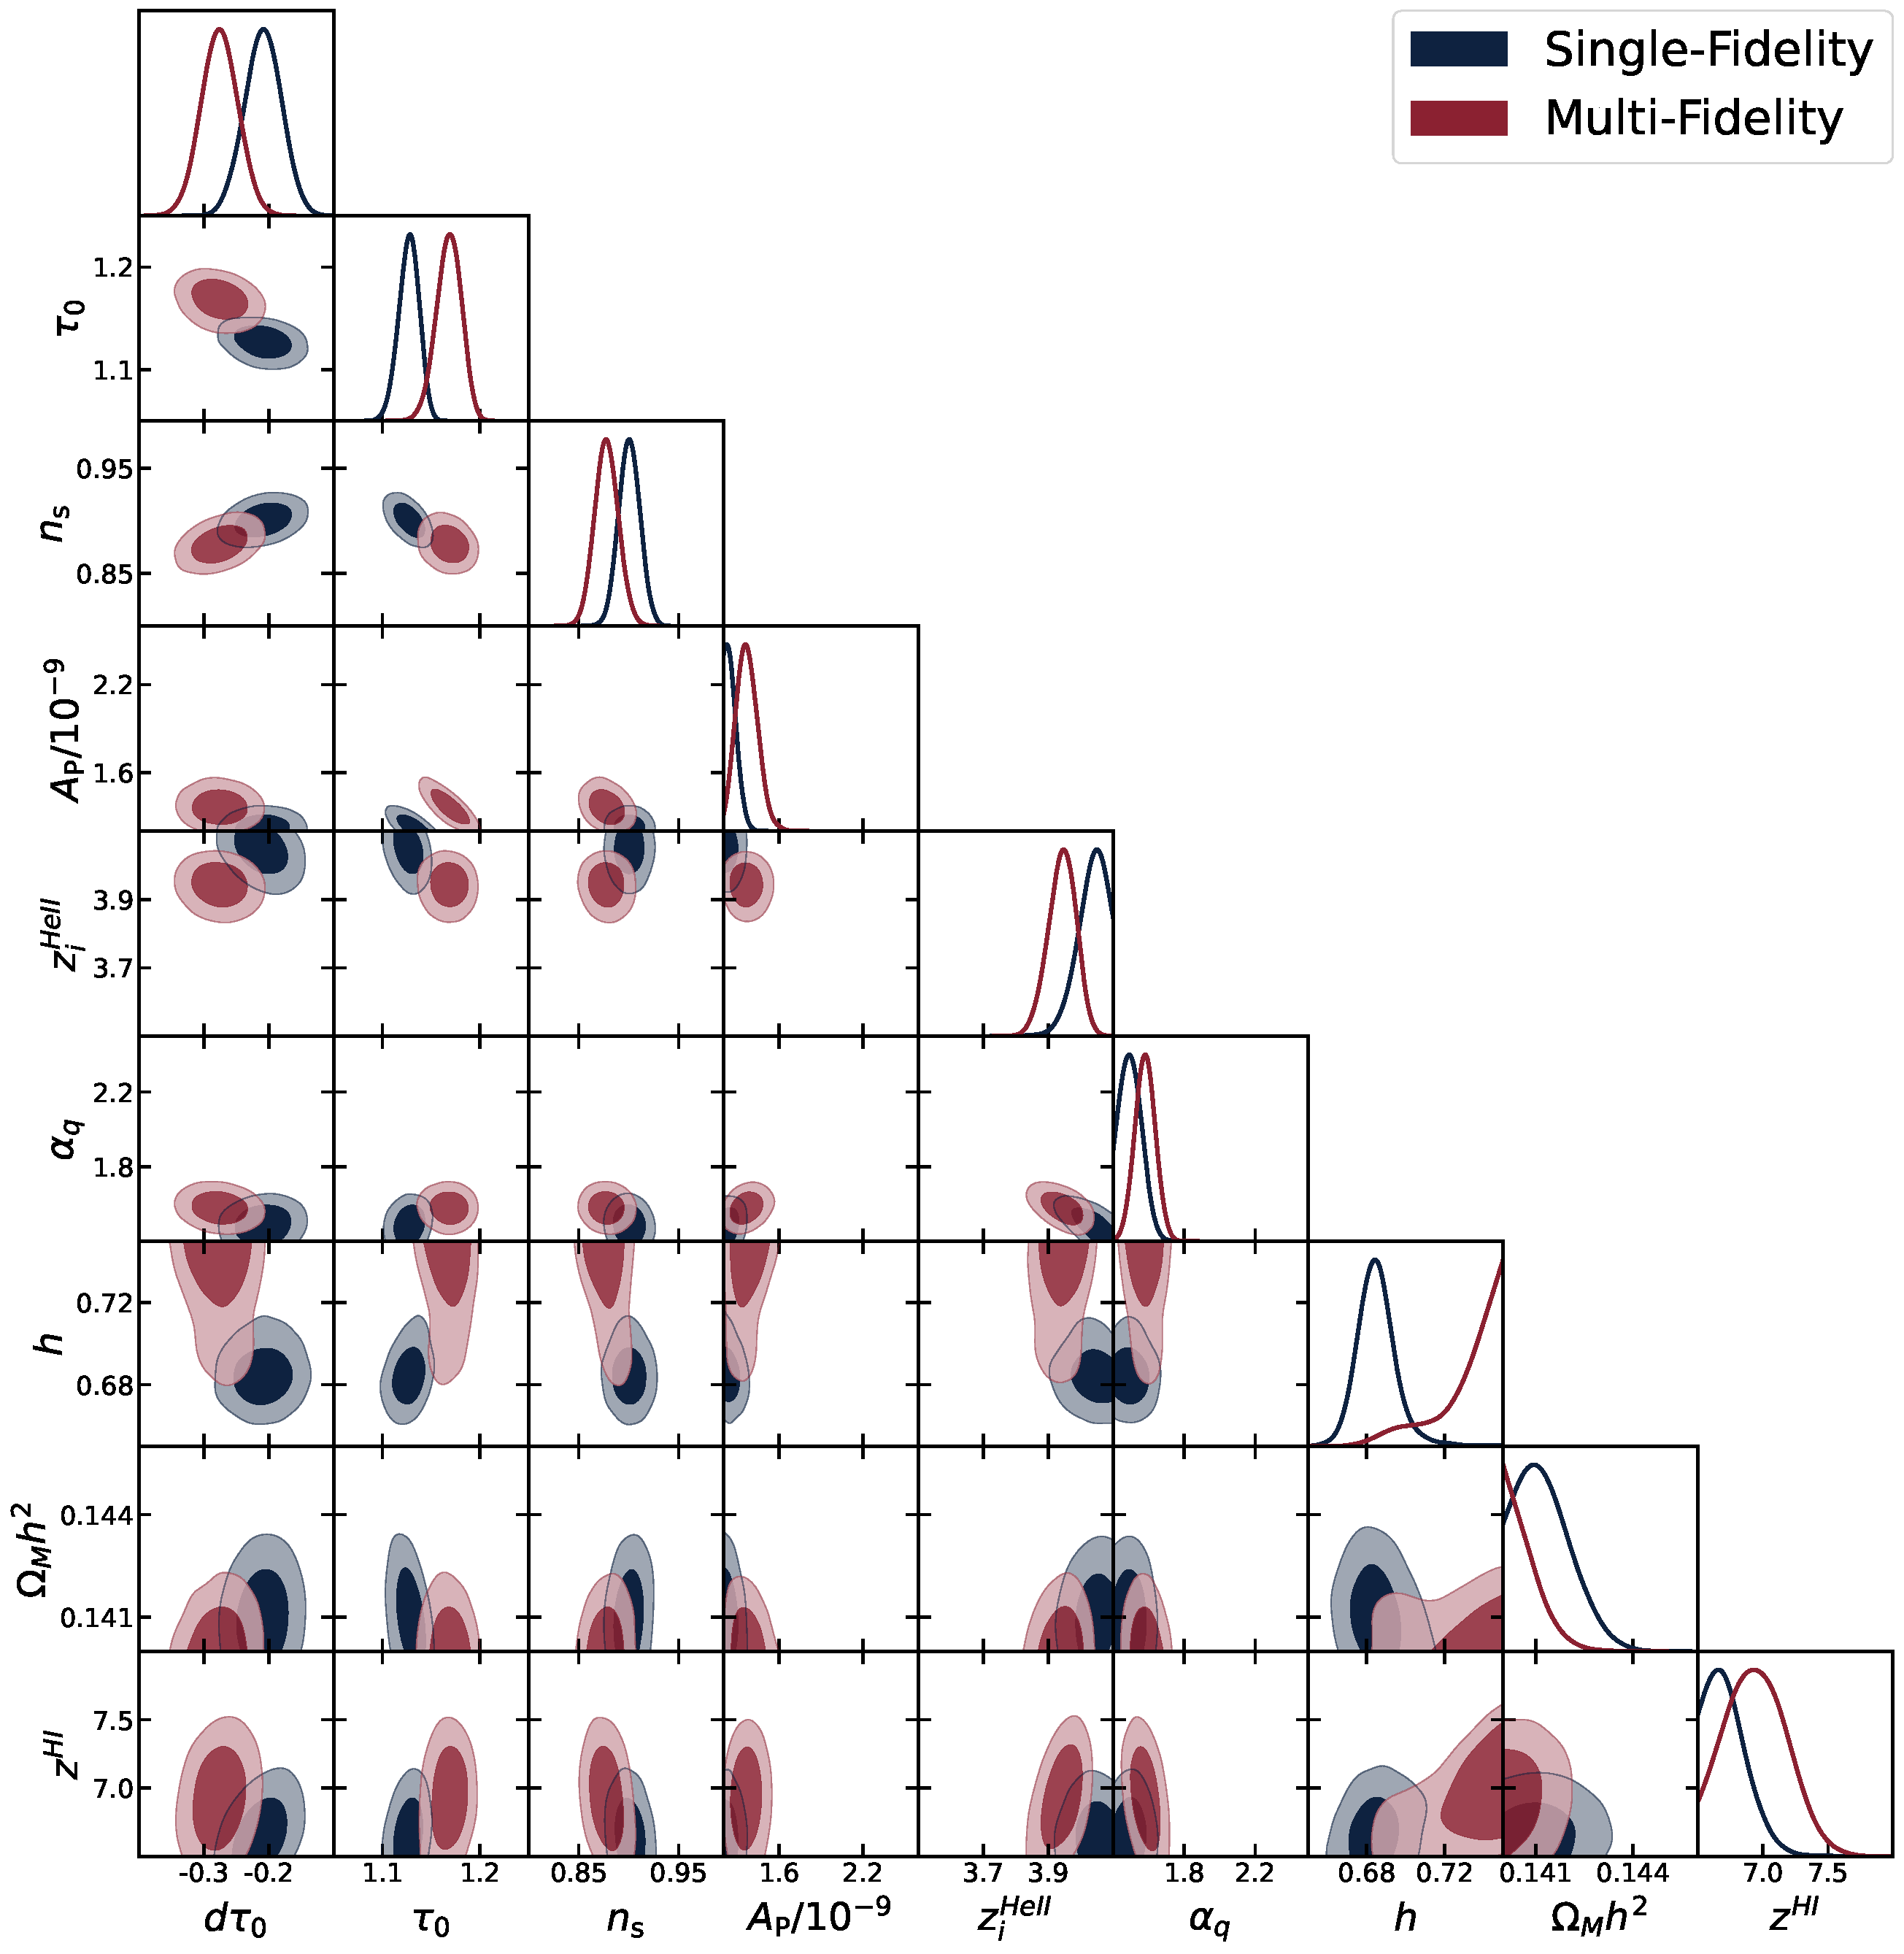
\includegraphics[width=\textwidth]{figures/sfemu_corner.pdf}
%     \caption{\label{fig:sfemu_corner}
%     Posteriors for chains run with a single-fidelity (black) and a multi-fidelity (red) emulator.
%     Both chains use the flux power and mean temperature, and have no priors.
%     }
% \end{figure}

% In this section, we present results from a chain using a single-fidelity emulator.
% This predicts the flux power and mean temperature at the resolution of our LF simulation suite.
% Figure~\ref{fig:sfemu_corner} shows parameters posteriors for the single-fidelity emulator (black) and, for comparison, the multi-fidelity emulator (red).
% Parameters excluded from Figure~\ref{fig:sfemu_corner} were unaffected by the choice of single- or multi-fidelity.

% Thus, the parameters shown are all affected by this change, and include: the mean flux rescaling parameters, $n_P$, $A_p$, the start of He~{\sc ii} reionization, $\alpha_q$, $h$, $\Omega_M h^2$, and the midpoint of H~{\sc i} reionization.
% The first four of these are consistent with each other; the single-fidelity prefers a larger slope and smaller amplitude for the mean flux and primordial power.
% The two He~{\sc ii} reionization parameters and midpoint of H~{\sc i} reionization are correlated, so the shift in these may be due to those degeneracies.
% Also correlated are $h$ and $\Omega_M h^2$, which are both significantly affected in the single-fidelity chain.
% The main way in which $h$ alters the flux power is through the mean flux, shifting the matter power and thus the flux power.
% The change in $h$ is therefore not entirely surprising, given the change in the mean flux rescaling parameters.

% The results for the single-fidelity are similar to those when the lowest redshift is omitted, Figure~\ref{fig:zrange}, especially for $h$, $A_p$, and z$^{\text{H~{\sc i}}}$.
% The results for the single-fidelity are also similar to those when the largest scales are omitted, Figure~\ref{fig:krange}, especially for $h$, $n_P$, and $\Omega_M h^2$.
% In combination, this may indicate that the single-fidelity is underfitting the largest scales and lowest redshifts.

% --------------------------------------------------------------------------------------------------
\section{BOSS DR9 Data}\label{sec:dr9_results}
\begin{figure}
    \centering
    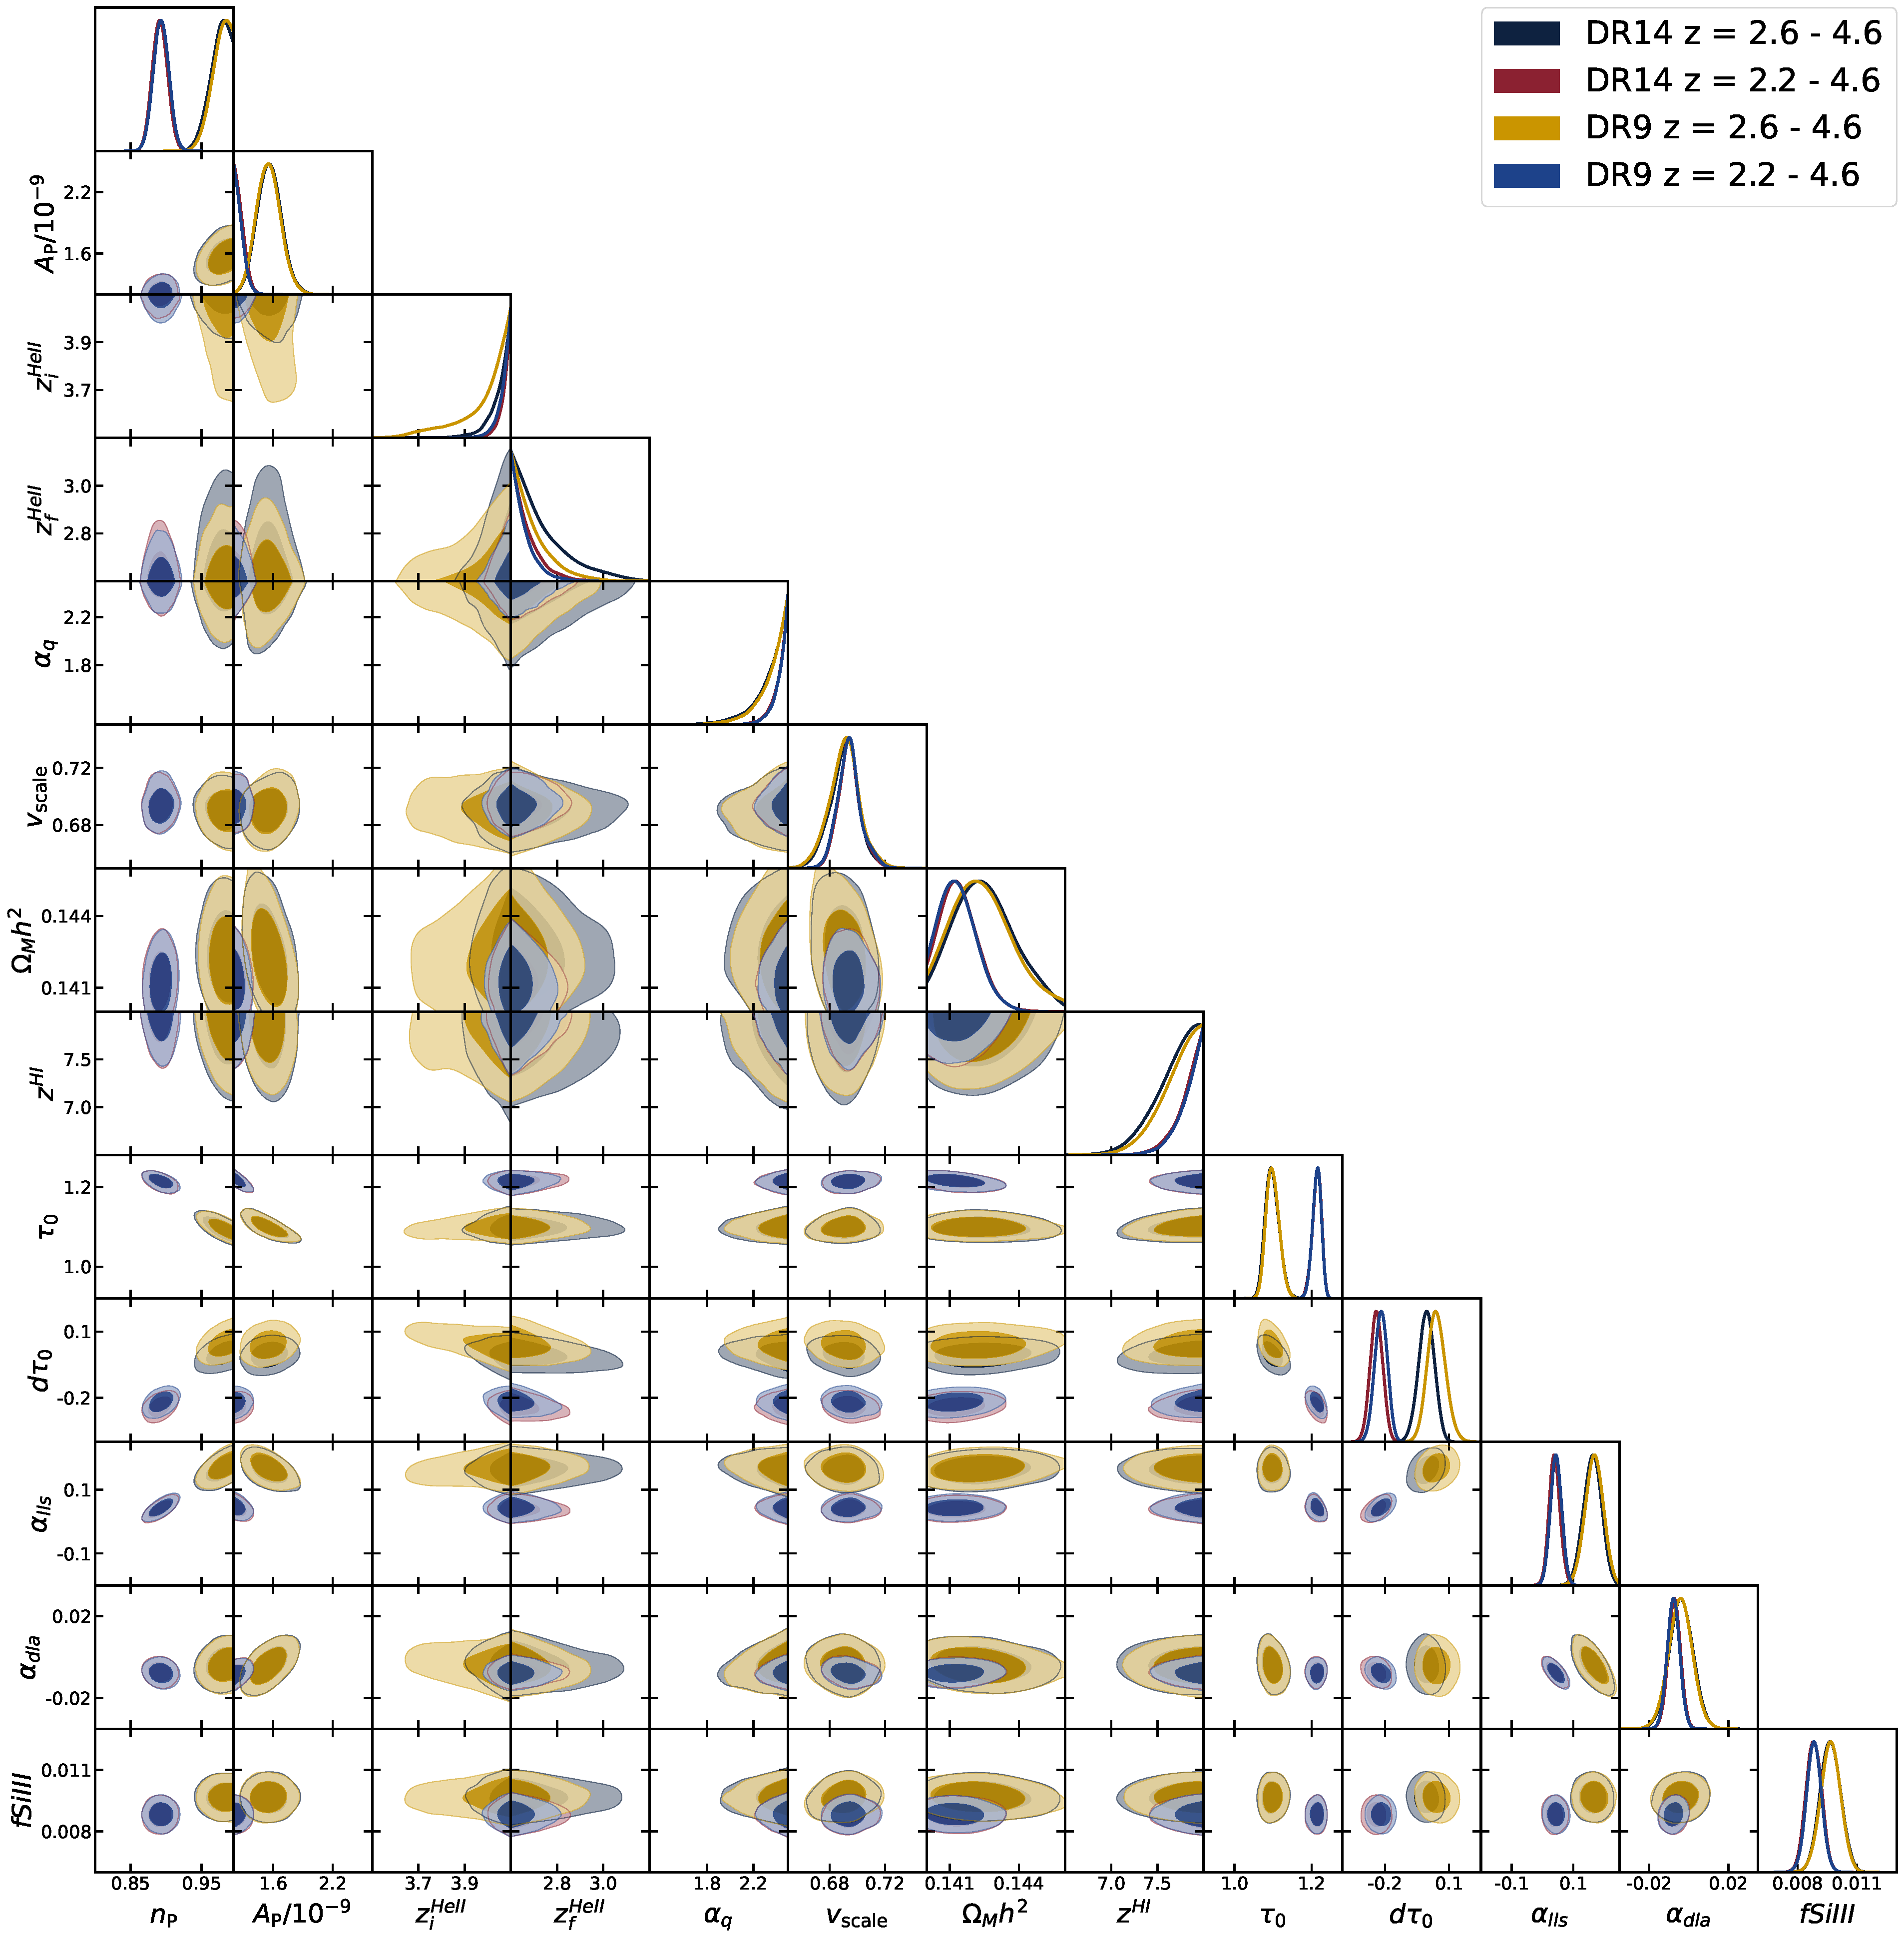
\includegraphics[width=\textwidth]{figures/dr9_allp_corner.pdf}
    \caption{\label{fig:dr9_corner}
    Posteriors for chains run using observations from the earlier SDSS data release, DR9, for the reduced redshift range (gold) and full redshift range (blue), compared to our main chains using DR14 with the reduced redshift range (black) and full redshift range (red).
    }
\end{figure}

In this section we compare posteriors obtained using the flux power spectrum from Ref.~\cite{2013A&A...559A..85P}, which is based on BOSS DR9 quasar spectra.
Figure~\ref{fig:dr9_corner} shows the posteriors for chains run with DR14, with both reduced and full redshift ranges, and chains with DR9, again with the reduced and full redshift ranges. We show chains using only the flux power spectrum likelihood, to emphasise any differences between the datasets.

\textbf{The tension between $z <2.6$ and $z \geq 2.6$ remains in DR9, and the parameter shifts by dropping the lowest redshift bins are similar. DR9 measures an $A_P$ very similar to DR14, which would continue to imply a low $\sigma_8$. 
The $\tau_0$ posteriors are also similar. The best-fit helium reionization model is similar in both datasets.}

\textbf{The largest parameter changes are $\approx 2\sigma$ shift in the posterior values of $n_P$ and $d\tau_0$. DR9 prefers a lower $n_P$, around $n_P = 0.95$. DR9 is still consistent with the Planck value of $n_P = 0.97$, and marginally consistent with the upper limit of our emulator, $n_P = 0.995$. DR9 also prefers a higher $d\tau_0$, again at about $2\sigma$. This shift is plausibly because of the inclusion of high redshift data in DR14, which would provide a longer redshift lever to measure $d\tau_0$. Interestingly, the shift in $n_P$ between DR9 and DR14 in our analysis is similar to the shift in $n_s$ between Refs.~\cite{2020JCAP...04..038P} and \cite{2015JCAP...11..011P}. However, the measured posterior for $d\tau_0$ in Ref.~\cite{2015JCAP...11..011P} from DR9 is similar to our result from \textit{DR14}. Ref.~\cite{2020JCAP...04..038P} do not report a posterior value for $d\tau_0$, but our results suggest it may be larger.}

\textbf{Although DR14 includes many more quasars, the covariance matrix is often dominated by systematic error. At $z=2.6$ DR14 and DR9 have very similar errors, while DR14 has smaller measurement uncertainty at $z \geq 3$. The posterior uncertainties for DR9 are for most parameters similar to those for DR14. There are some exceptions: $z_{HI}$ and $z_i^{HeII}$, which measure specifically high redshift effects, are marginally constrained in DR14 yet unconstrained in DR9.}

\section{IGM Temperature at Mean Density Posteriors}\label{sec:t0-only}

\begin{figure}
    \centering
    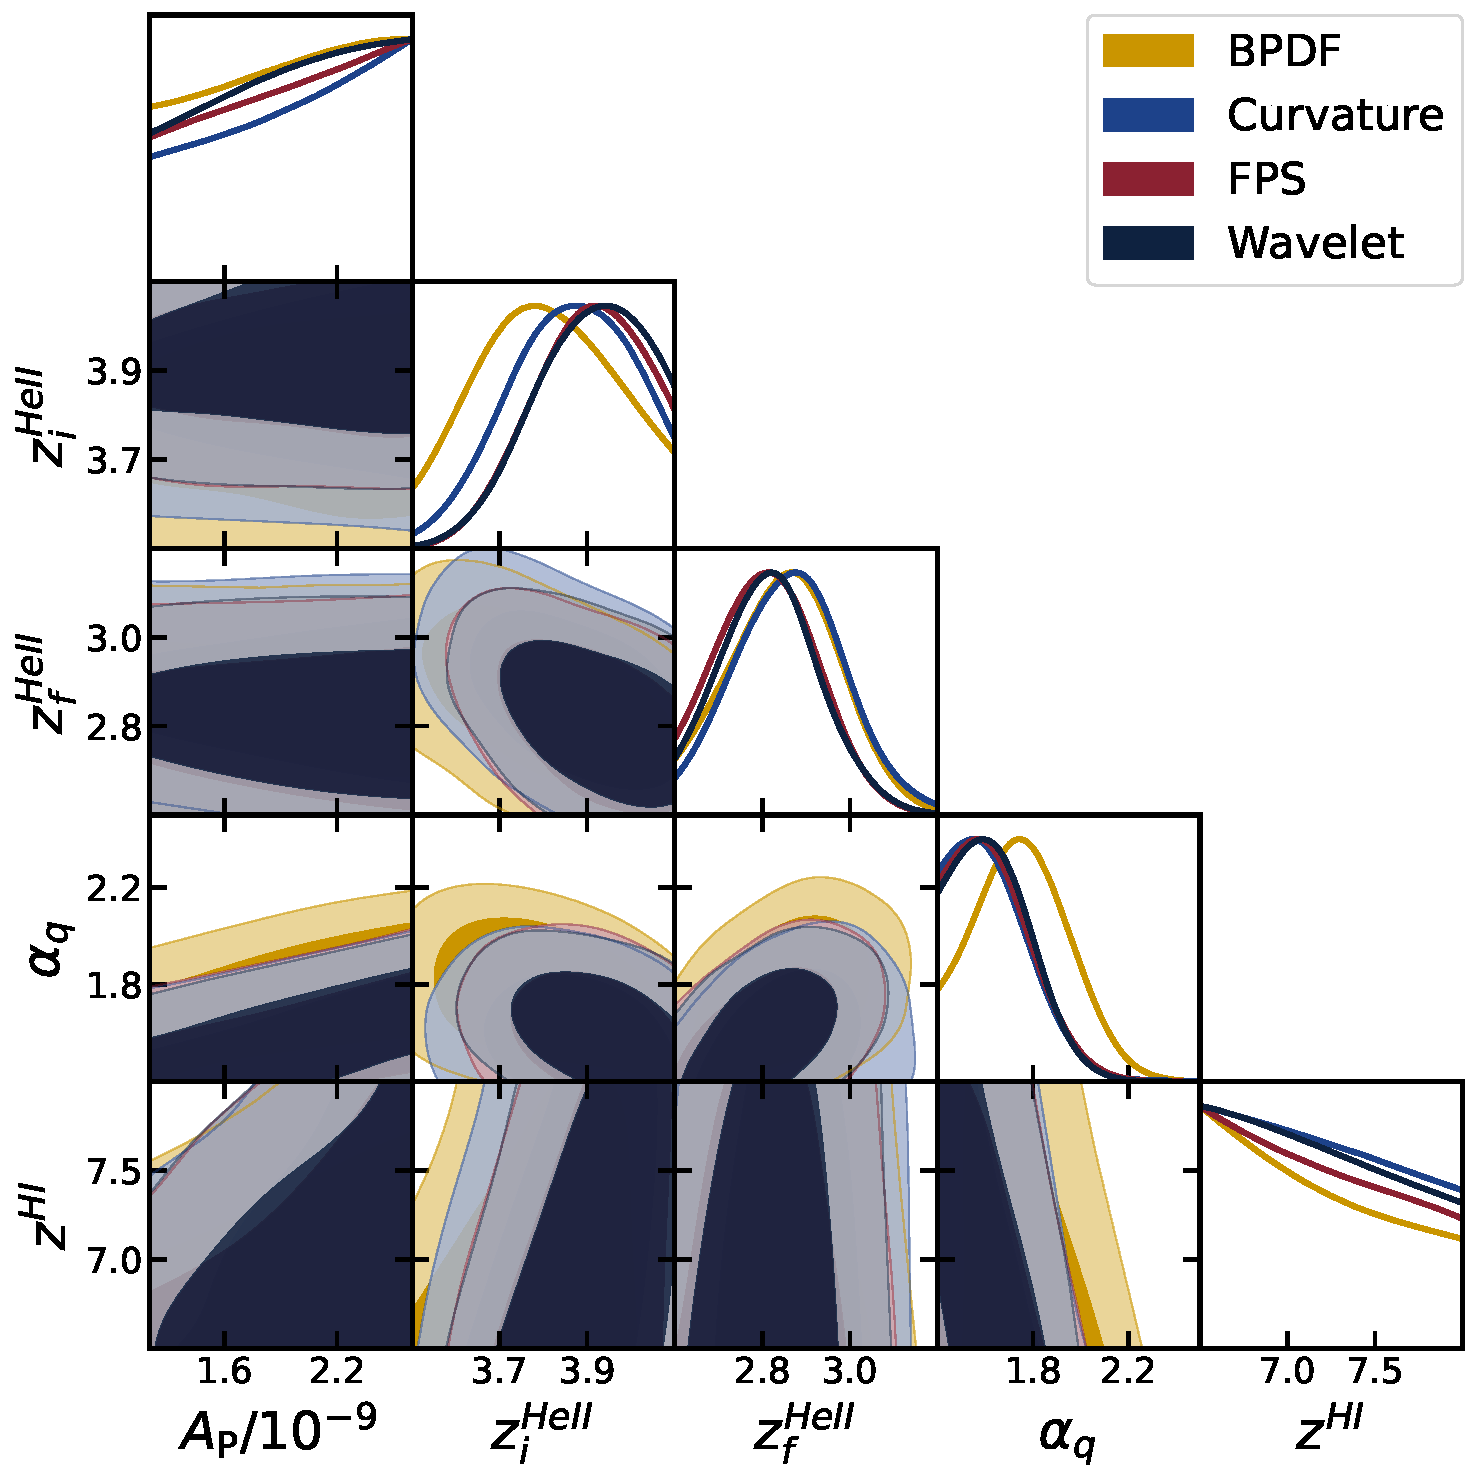
\includegraphics[width=\textwidth]{figures/datasets_t0_corner.pdf}
    \caption{\label{fig:t0_datasets}
    Posteriors for chains run with only the IGM temperature likelihood.
    Shown are chains using each of the four observational measurements of the IGM temperature: using the flux power spectrum (blue), using the Doppler width distribution (BPDF, yellow), using the curvature statistic (red), and using a wavelet decomposition (black).
    The main results of this work use the flux power derived IGM temperatures.
    }
\end{figure}

In this section, we present results from chains run using only the IGM temperature likelihood.
Shown in Figure~\ref{fig:t0_datasets} are four chains, each using one of the observational measurements of the IGM temperature at mean density, derived from different \lya forest summary statistics: the flux power spectrum, the Doppler width distribution, the curvature statistic, and a wavelet decomposition.
Most of the cosmology parameters are entirely unconstrained by the IGM temperature and are omitted from the Figure.
We show $A_p$ for reference.
The three He~{\sc ii} reionization parameters are well constrained by the IGM temperature history.
There is very little difference between the different IGM temperature observations, with the BPDF derived temperature differing the most, specifically preferring a later start to He~{\sc ii} reionization, and less heating, corresponding to a lower IGM temperature.
However, differences are well within $1\sigma$.

The midpoint of H~{\sc i} reionization has a marginal preference for a late midpoint, but is very weakly constrained.
The IGM temperature provides information on $z_{HI}$ as the IGM cools from the completion of H~{\sc i} reionization, setting the temperature before the onset of helium reionization.
Incorporating measurements of the IGM temperature at $z > 3.8$  \cite[e.g.~][]{2023arXiv230402038G} could substantially improve these constraints and we may do so in future work.

\section{Full Posteriors}
\label{sec:full_posteriors}
\begin{figure}
    \centering
    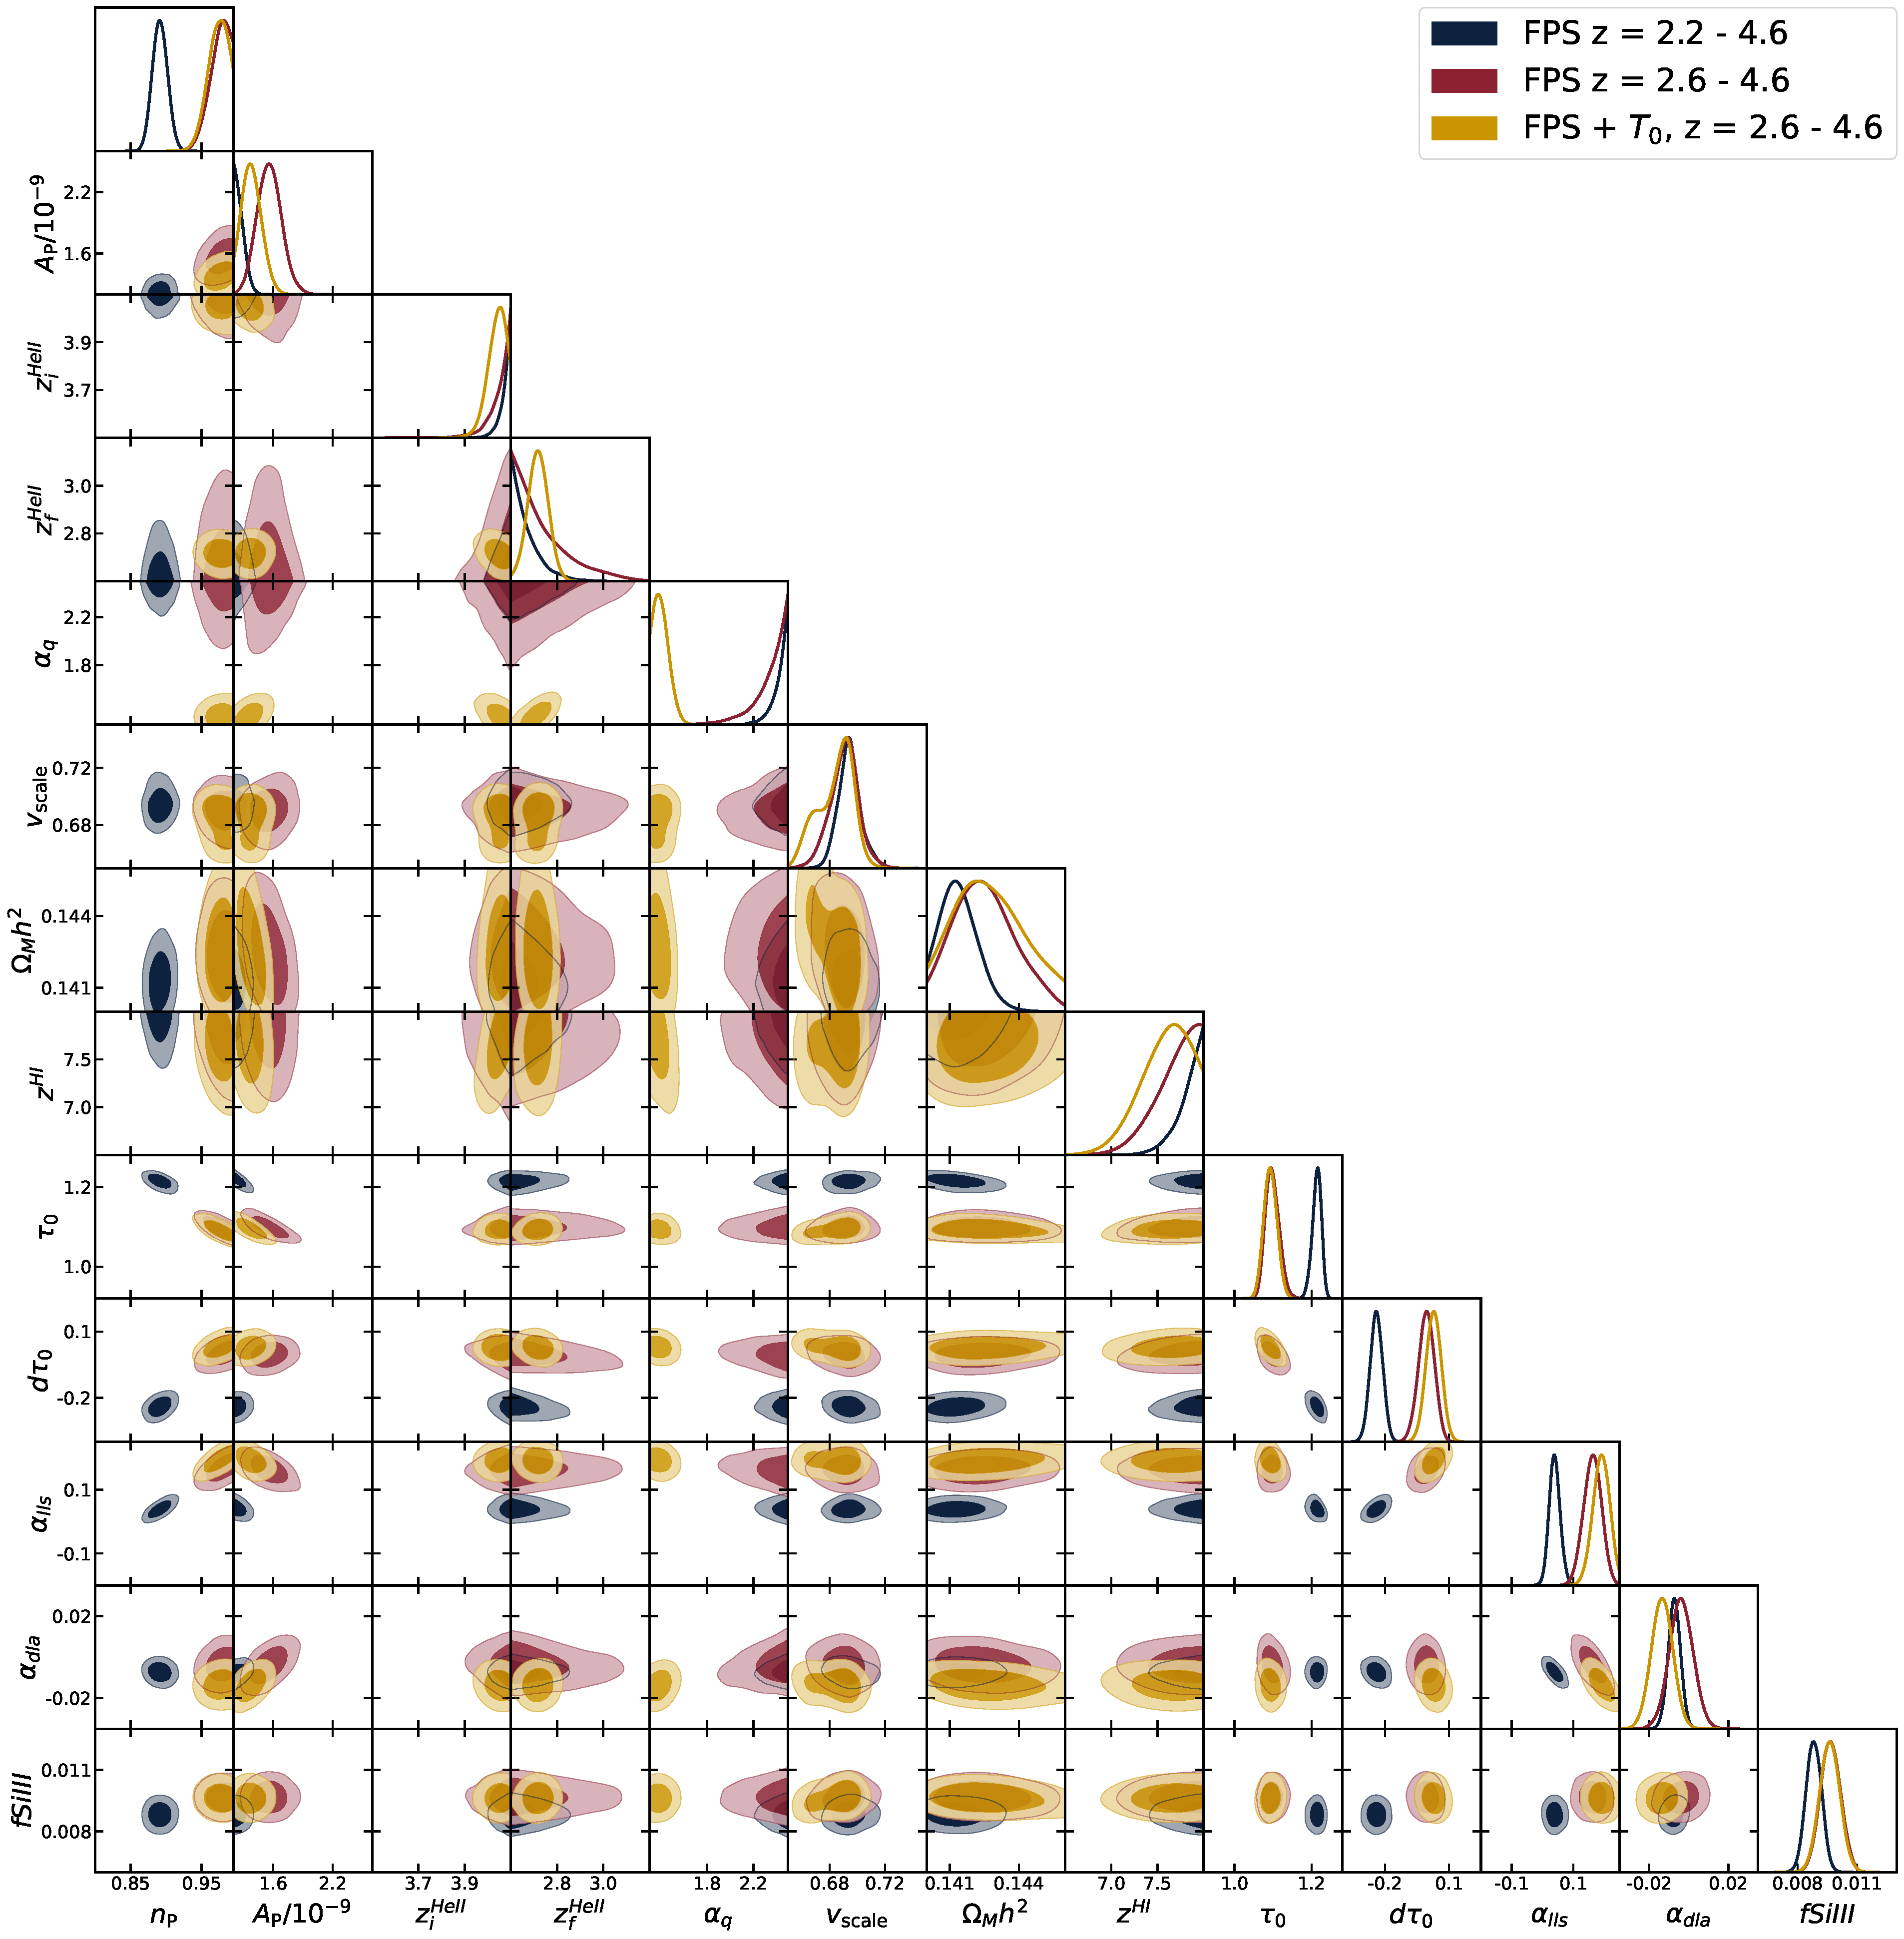
\includegraphics[width=\textwidth]{figures/allp_corner.pdf}
    \caption{\label{fig:full_posterior}
    Posteriors for the full set of simulation parameters, both cosmological and astrophysical.
    Shown are the same chains from the figures in Section~\ref{sec:results}, thus the correlations between the the parameters in Figure~\ref{fig:cosmo_corner} and those in Figure~\ref{fig:astro_corner} are the only new information here. `FPS $z=2.2-4.6$' (gold) uses the full redshift range eBOSS flux power spectrum dataset, `FPS $z=2.6-4.6$' (blue) uses a reduced redshift range eBOSS dataset flux power spectrum dataset, which removes the internal tension (Section~\ref{sec:tension}).
    The third chain, `FPS $+T_0, z=2.6-4.6$' (red), uses the limited range eBOSS dataset but adds the IGM temperature constraints.
    }
\end{figure}

Figure~\ref{fig:full_posterior} presents the full posteriors, including the correlations between the cosmology and astrophysics parameter sets, using the same chains discussed extensively in Section~\ref{sec:results}.
Correlations are discussed in Section~\ref{sec:correlations}.
%For the chains run using both the mean temperature and flux power, the main correlations are: a slightly negative correlation between $n_P$ and $A_p$; a negative correlation between z$^{\text{He~{\sc ii}}}_i$ and both $\alpha_q$ and z$^{\text{He~{\sc ii}}}_f$; a positive correlation between z$^{\text{He~{\sc ii}}}_i$ and z$^{\text{H~{\sc i}}}$; a negative correlation between $\alpha_q$ and z$^{\text{H~{\sc i}}}$; and a positive correlation between $\alpha_q$ and z$^{\text{He~{\sc ii}}}_f$.

%The only correlation between astrophysics and cosmology is a positive correlation between $A_p$ and $\alpha_q$.
%This may indicate that a larger $\alpha_q$ (which corresponds to less heating) is appropriate when the primordial power spectrum amplitude is larger, which leads to more structure.



% --------------------------------------------------------------------------------------------------
% --------------------------------------------------------------------------------------------------
% --------------------------------------------------------------------------------------------------
% --------------------------------------------------------------------------------------------------
% --------------------------------------------------------------------------------------------------


% \subsection{Reduced Redshift Range}\label{sec:reducedz}

% In this section, we present results from chains run using a reduced range of redshifts.
% Both chains are run using the multi-fidelity emulator, with both the mean temperature and flux power likelihoods.
% One chain is run with the lowest redshift bin ($z=2.2$) omitted, while another chain is run leaving out the three highest redshift bins ($z=4.2-4.6$).
% The results of these chains are shown in Figure~\ref{fig:krange} (red and yellow), along with a chain using the full range of redshifts (black).

% Most of the parameters are relatively stable between these two chains: $n_P$, $A_p$, the three He~{\sc ii} reionization parameters, $\Omega_M h^2$, and $\epsilon_{AGN}$.
% The midpoint of reionization redshift, z$^{\text{H~{\sc i}}}$, is affected by the choice of redshifts to include.
% When the high redshifts are omitted, the midpoint is pushed later, as information on the asymptotic cooling after reionization is lost.
% When the low redshift is omitted, the midpoint is also shifted lower, though this is likely through the degeneracy with the start of He~{\sc ii} reionization.

% When the low redshift is omitted, the value for $h$ shifts towards the middle of the range.
% This is an indication that the value for $h$ in Figure~\ref{fig:sfemu_corner} (single-fidelity, LF results) is partially driven by possible underfitting of the $z=2.2$ flux power and mean temperature.
% These results indicate that the full redshift range used in this work is worth including.

% \begin{figure}
%     \centering
%     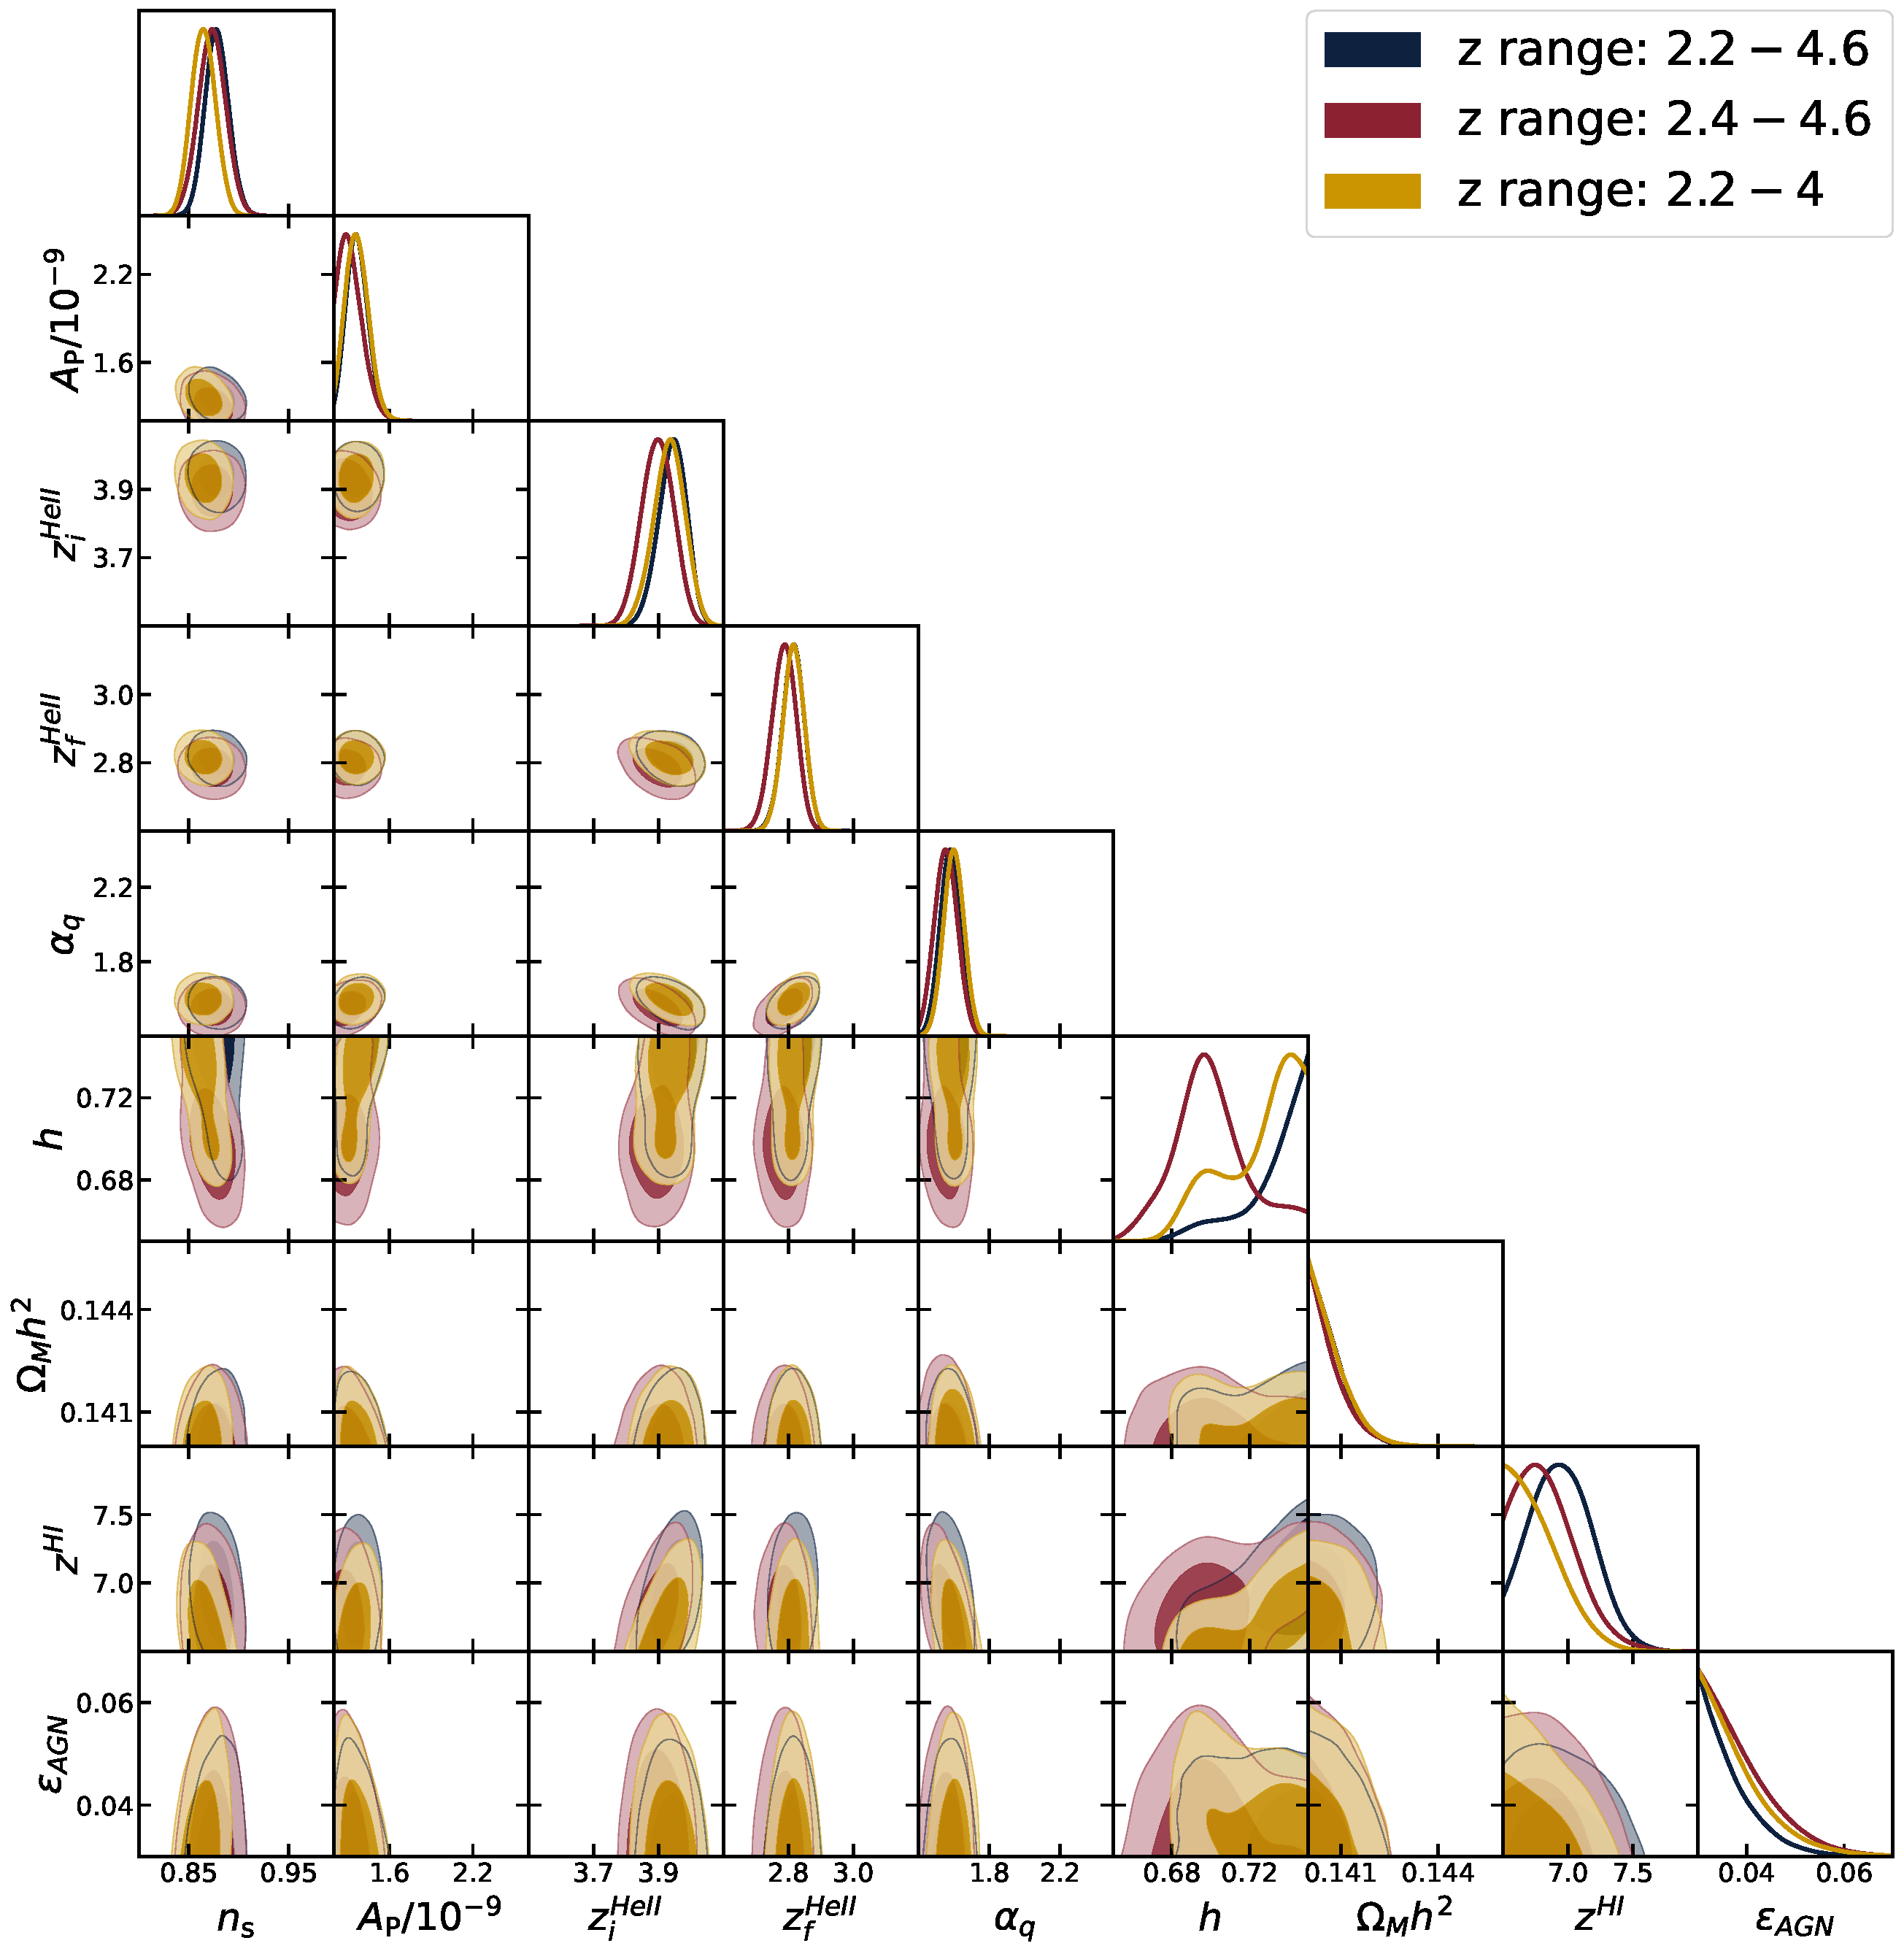
\includegraphics[width=\textwidth]{figures/zscale_corner.pdf}
%     \caption{\label{fig:zrange}
%     Posteriors for chains run with reduced ranges for the redshifts used in the flux power and mean temperature likelihoods.
%     Shown are a chain without the lowest redshift bin (red), a chain without highest three redshift bins (yellow), and a chain using all redshifts (black), for comparison.
%     }
% \end{figure}

% --------------------------------------------------------------------------------------------------
% --------------------------------------------------------------------------------------------------
% --------------------------------------------------------------------------------------------------
% --------------------------------------------------------------------------------------------------
% --------------------------------------------------------------------------------------------------


% \subsection{Reduced Scale Range}\label{sec:reducedk}

% In this section, we present results from chains run using a reduced range of scales.
% Both chains are run using the multi-fidelity emulator, the full redshift range, with both the mean temperature and flux power likelihoods.
% One chain is run with the three largest scales (three smallest $k$) omitted.
% Note that this is roughly the scales where systematics in the continuum dominate over statistical error.
% Another chain is run leaving out the five smallest scales (five largest $k$).
% \spb{It would be nice to see a chain which excludes all data where the spectrograph resolution dominates. Unfortunately for $z = 2.4$, this is $k > 0.008672$ s/km, which is a lot of the data. Probably the constraints just become poor, but it would be nice to see it anyway.}.
% The results of these chains are shown in Figure~\ref{fig:krange} (red and yellow), along with a chain using the full range of scales (black).

% Several parameters are relatively stable between these two chains: $A_p$, the three He~{\sc ii} reionization parameters, and $\epsilon_{AGN}$.
% The value for $n_P$ is slightly higher when the largest scales are omitted, highlighting the importance of the large scales, and thus the volume used in our simulations.
% The midpoint of reionization redshift, z$^{\text{H~{\sc i}}}$, is not well constrained when the large scales are omitted, likely as a result of the higher value of $n_P$.
% When the large scales are omitted $\Omega_M h^2$ shifts off of the edge slightly, and this is accompanied by a secondary mode strengthening in $h$.
% This may indicate that the value for $h$ and $\Omega_M h^2$ are partially driven by overfitting of small scales, at the expense of large scales.
% These results indicate that the increased volume of the simulations used in this work have helped the analysis, by better resolving the largest scales.

% \begin{figure}
%     \centering
%     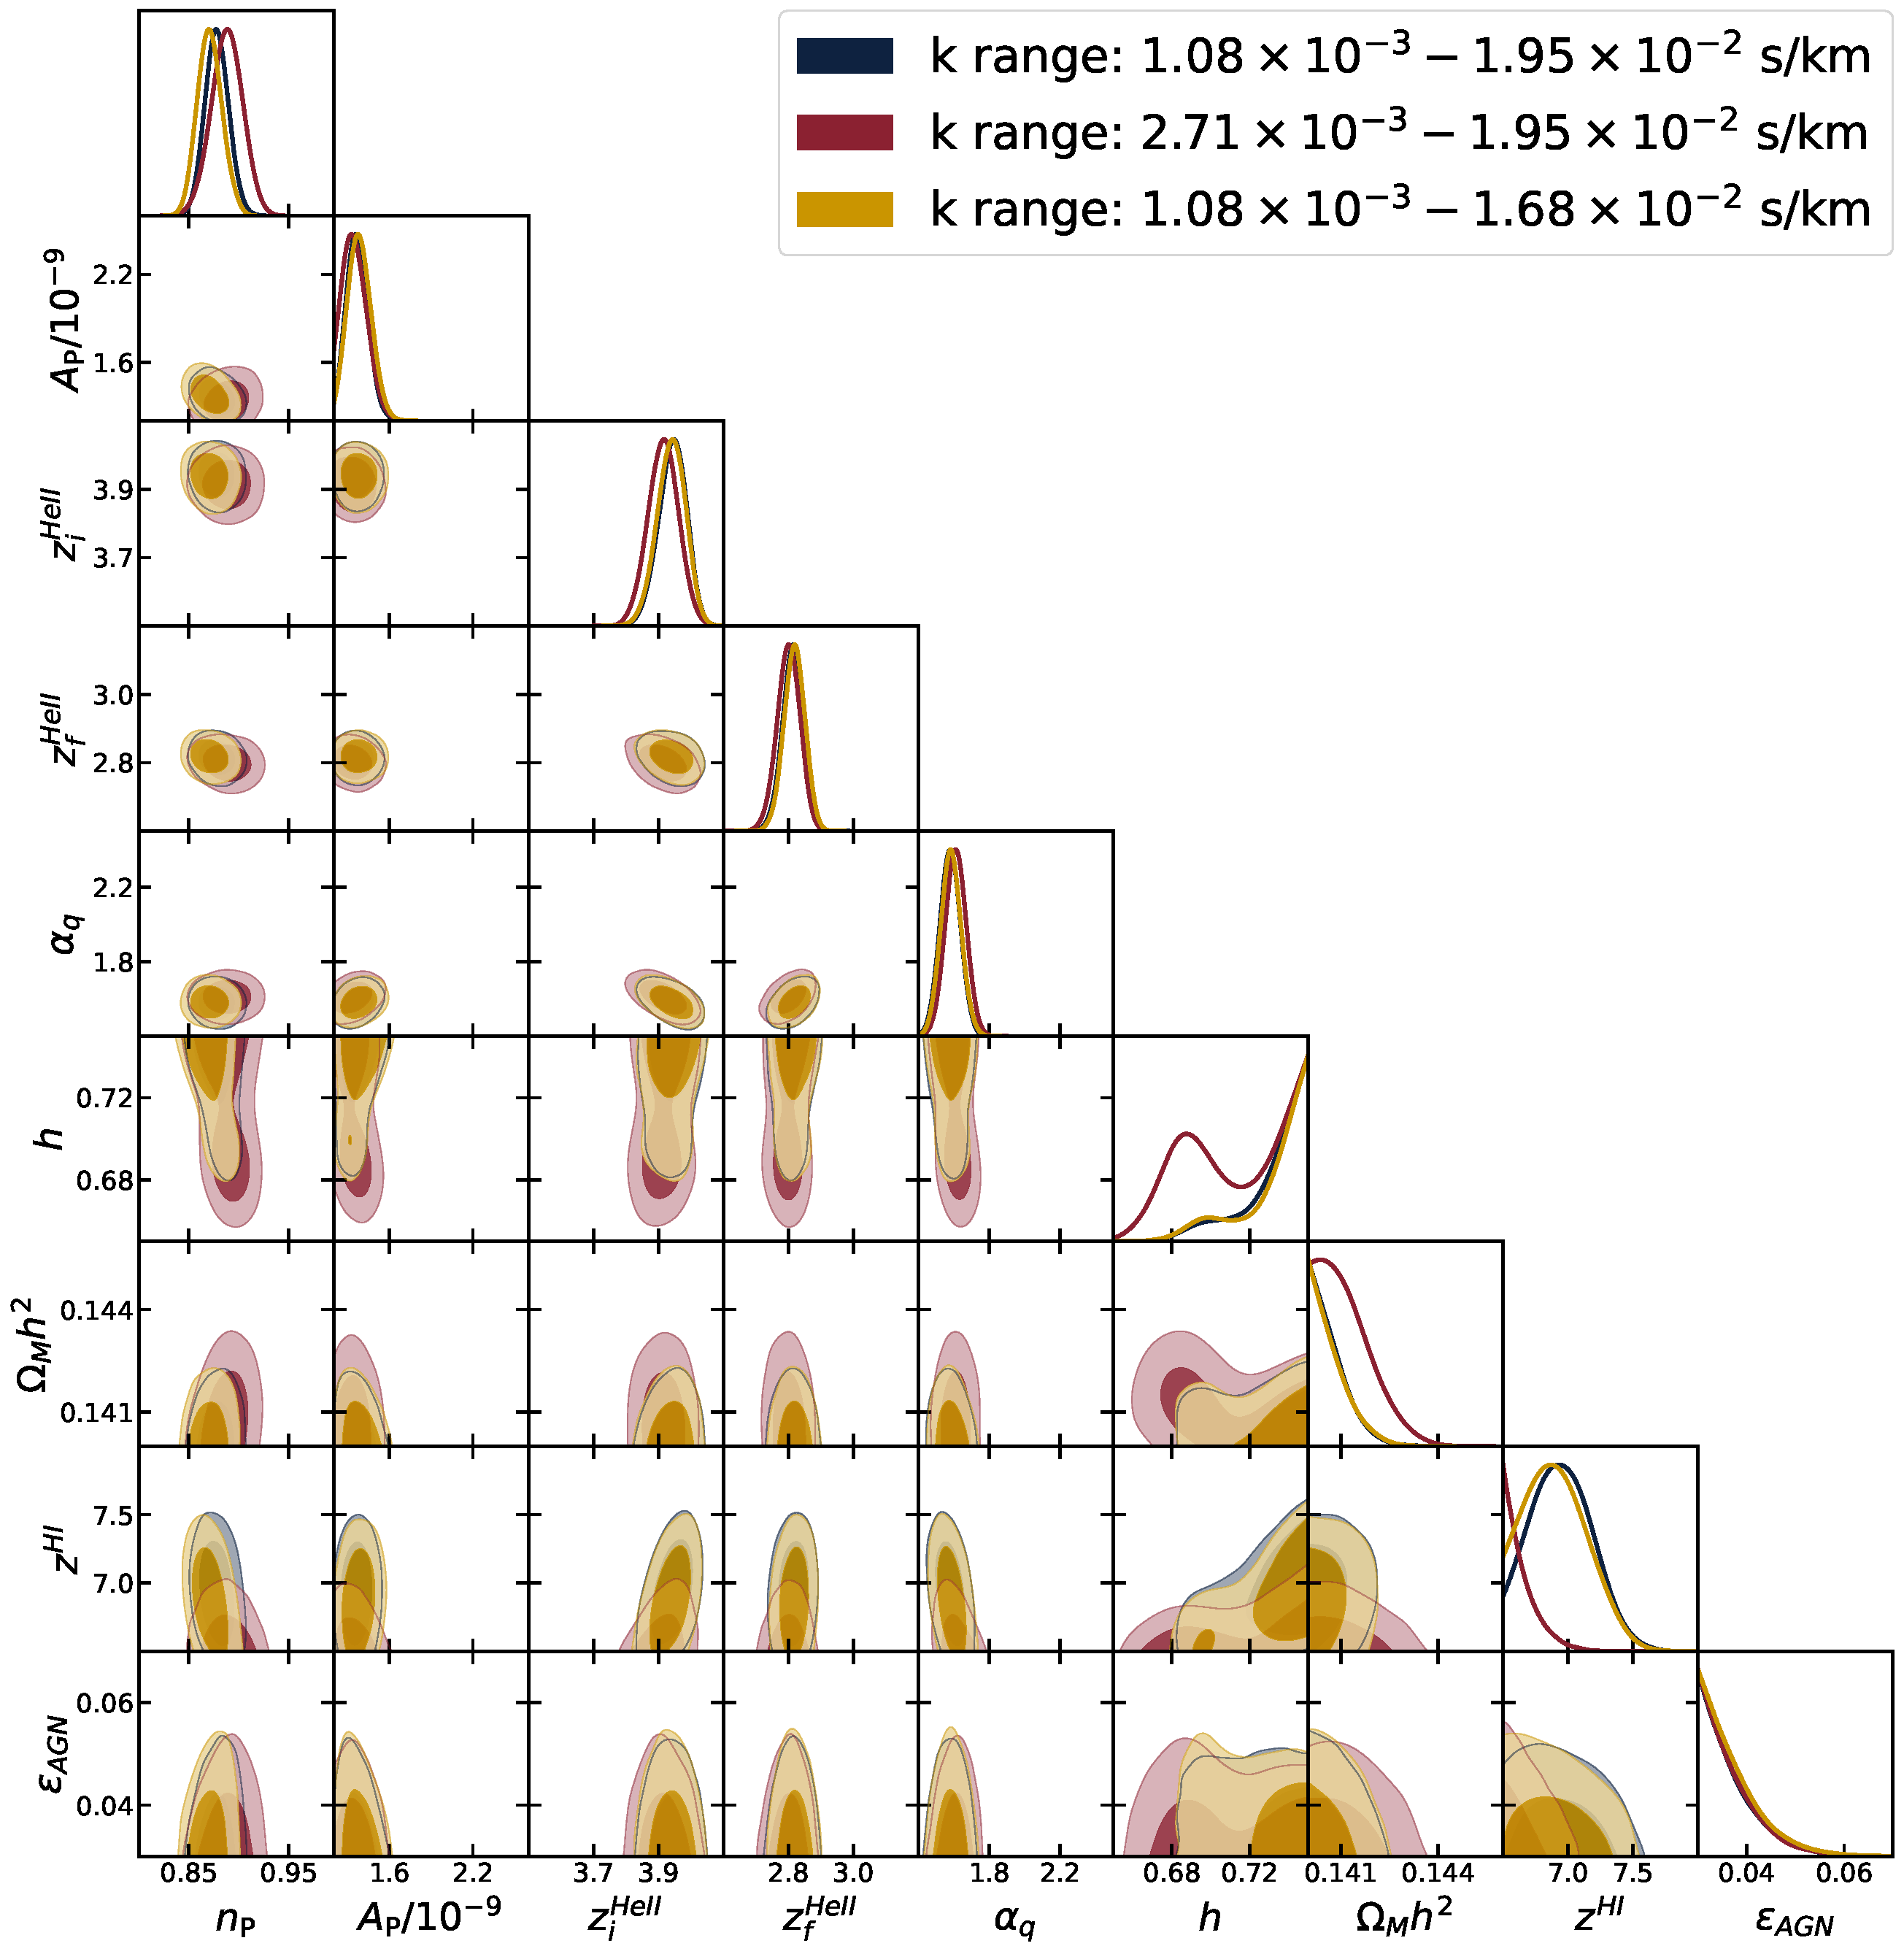
\includegraphics[width=\textwidth]{figures/kscale_corner.pdf}
%     \caption{\label{fig:krange}
%     Posteriors for chains run with reduced ranges for the scales used in the flux power likelihood.
%     Shown are a chain without the three largest scales (red), a chain without the five smallest scales (yellow), and a chain using all scales (black), for comparison.
%     }
% \end{figure}
